\documentclass[twoside]{book}

% Packages required by doxygen
\usepackage{fixltx2e}
\usepackage{calc}
\usepackage{doxygen}
\usepackage[export]{adjustbox} % also loads graphicx
\usepackage{graphicx}
\usepackage[utf8]{inputenc}
\usepackage{makeidx}
\usepackage{multicol}
\usepackage{multirow}
\PassOptionsToPackage{warn}{textcomp}
\usepackage{textcomp}
\usepackage[nointegrals]{wasysym}
\usepackage[table]{xcolor}

% Font selection
\usepackage[T1]{fontenc}
\usepackage[scaled=.90]{helvet}
\usepackage{courier}
\usepackage{amssymb}
\usepackage{sectsty}
\renewcommand{\familydefault}{\sfdefault}
\allsectionsfont{%
  \fontseries{bc}\selectfont%
  \color{darkgray}%
}
\renewcommand{\DoxyLabelFont}{%
  \fontseries{bc}\selectfont%
  \color{darkgray}%
}
\newcommand{\+}{\discretionary{\mbox{\scriptsize$\hookleftarrow$}}{}{}}

% Page & text layout
\usepackage{geometry}
\geometry{%
  a4paper,%
  top=2.5cm,%
  bottom=2.5cm,%
  left=2.5cm,%
  right=2.5cm%
}
\tolerance=750
\hfuzz=15pt
\hbadness=750
\setlength{\emergencystretch}{15pt}
\setlength{\parindent}{0cm}
\setlength{\parskip}{3ex plus 2ex minus 2ex}
\makeatletter
\renewcommand{\paragraph}{%
  \@startsection{paragraph}{4}{0ex}{-1.0ex}{1.0ex}{%
    \normalfont\normalsize\bfseries\SS@parafont%
  }%
}
\renewcommand{\subparagraph}{%
  \@startsection{subparagraph}{5}{0ex}{-1.0ex}{1.0ex}{%
    \normalfont\normalsize\bfseries\SS@subparafont%
  }%
}
\makeatother

% Headers & footers
\usepackage{fancyhdr}
\pagestyle{fancyplain}
\fancyhead[LE]{\fancyplain{}{\bfseries\thepage}}
\fancyhead[CE]{\fancyplain{}{}}
\fancyhead[RE]{\fancyplain{}{\bfseries\leftmark}}
\fancyhead[LO]{\fancyplain{}{\bfseries\rightmark}}
\fancyhead[CO]{\fancyplain{}{}}
\fancyhead[RO]{\fancyplain{}{\bfseries\thepage}}
\fancyfoot[LE]{\fancyplain{}{}}
\fancyfoot[CE]{\fancyplain{}{}}
\fancyfoot[RE]{\fancyplain{}{\bfseries\scriptsize Generated by Doxygen }}
\fancyfoot[LO]{\fancyplain{}{\bfseries\scriptsize Generated by Doxygen }}
\fancyfoot[CO]{\fancyplain{}{}}
\fancyfoot[RO]{\fancyplain{}{}}
\renewcommand{\footrulewidth}{0.4pt}
\renewcommand{\chaptermark}[1]{%
  \markboth{#1}{}%
}
\renewcommand{\sectionmark}[1]{%
  \markright{\thesection\ #1}%
}

% Indices & bibliography
\usepackage{natbib}
\usepackage[titles]{tocloft}
\setcounter{tocdepth}{3}
\setcounter{secnumdepth}{5}
\makeindex

% Hyperlinks (required, but should be loaded last)
\usepackage{ifpdf}
\ifpdf
  \usepackage[pdftex,pagebackref=true]{hyperref}
\else
  \usepackage[ps2pdf,pagebackref=true]{hyperref}
\fi
\hypersetup{%
  colorlinks=true,%
  linkcolor=blue,%
  citecolor=blue,%
  unicode%
}

% Custom commands
\newcommand{\clearemptydoublepage}{%
  \newpage{\pagestyle{empty}\cleardoublepage}%
}

\usepackage{caption}
\captionsetup{labelsep=space,justification=centering,font={bf},singlelinecheck=off,skip=4pt,position=top}

%===== C O N T E N T S =====

\begin{document}

% Titlepage & ToC
\hypersetup{pageanchor=false,
             bookmarksnumbered=true,
             pdfencoding=unicode
            }
\pagenumbering{alph}
\begin{titlepage}
\vspace*{7cm}
\begin{center}%
{\Large Framework L\+A\+MP }\\
\vspace*{1cm}
{\large Generated by Doxygen 1.8.12}\\
\end{center}
\end{titlepage}
\clearemptydoublepage
\pagenumbering{roman}
\tableofcontents
\clearemptydoublepage
\pagenumbering{arabic}
\hypersetup{pageanchor=true}

%--- Begin generated contents ---
\chapter{supinternet-\/orm}
\label{md_app_orm_README}
\hypertarget{md_app_orm_README}{}
{\ttfamily composer require droxyum/supinternet-\/orm dev-\/master} 

 \paragraph*{Create new connection to database\+:}

{\ttfamily \$\+Connection = new \textbackslash{}\hyperlink{namespaceORM}{O\+RM}\textbackslash{}Connection(host, database, username, password);}

\paragraph*{Create new Entity\+Manager\+:}

{\ttfamily \$\+Entity\+Manager = new \textbackslash{}\hyperlink{namespaceORM}{O\+RM}\textbackslash{}Entity\textbackslash{}Manager();} 

 \subsubsection*{Create new Entity \char`\"{}\+Post\char`\"{}\+:}


\begin{DoxyCode}
1 class Post extends Entity \{
2     const TABLE = 'posts';  //Table name
3     protected $id; //Id field (primary key)
4     protected $title; //Title field
5     protected $content; //Content field
6 
7     public function setId($id) \{ 
8         $this->id = $id;
9     \} 
10 
11     public function getId() \{ 
12         return $this->id;
13     \} 
14 
15     public function setTitle($title) \{ 
16         $this->title = $title;
17     \} 
18 
19     public function getTitle() \{ 
20         return $this->title;
21     \} 
22 
23     public function setContent($content) \{ 
24         $this->content = $content;
25     \} 
26 
27     public function getContent() \{ 
28         return $this->content;
29     \} 
30 
31 \}
\end{DoxyCode}


\#\#\# Insert new post\+: 
\begin{DoxyCode}
1 $Post = new \(\backslash\)Entity\(\backslash\)Post(); //New post
2 $Post->setTitle('My post title'); //Insert title
3 $Post->setContent('My post content'); //Insert content
4 $EntityManager->persist($Post); //Insert post in database
\end{DoxyCode}


\#\#\# Update post\+: 
\begin{DoxyCode}
1 $Post = new \(\backslash\)Entity\(\backslash\)Post(); //New post
2 $Post->setId(5); //Insert post's id
3 $Post->setTitle('New post title'); //Insert new title
4 $Post->setContent('New post content'); //Insert new content
5 $EntityManager->persist($Post); //Update post in database
\end{DoxyCode}


\#\#\# Remove post 
\begin{DoxyCode}
1 $Post = new \(\backslash\)Entity\(\backslash\)Post(); //New post
2 $Post->setId(5); //Insert post's id
3 $EntityManager->remove($Post); //Update post in database
\end{DoxyCode}


\#\#\# Find post 
\begin{DoxyCode}
1 $PostsRepository = $EntityManager->getRepository('Entity:Post'); //Get post repository
2 $PostsRepository->findAll(); //Find all post in database
\end{DoxyCode}


\#\#\# Find with relationship 
\begin{DoxyCode}
1 // New entity
2 //Category.php
3 class Category extends Entity 
4 \{ 
5     const TABLE = 'categories'; 
6     protected $id; 
7     protected $name; 
8 
9 
10     public function setId($id) \{ 
11         $this->id = $id;
12     \} 
13 
14     public function getId() \{ 
15         return $this->id;
16     \} 
17 
18     public function setName($name) \{ 
19         $this->name = $name;
20     \} 
21 
22     public function getName() \{ 
23         return $this->name;
24     \} 
25 
26 \}
27 
28 // Entity post created (Juste NanyToOne relation is available)
29 //Post.php
30 class Post extends Entity \{
31     // ...
32     protected $Categories;   // Join field on \(\backslash\)Entity\(\backslash\)Category
33     public function \_\_construct() \{
34         $this->Categories = new ManyToOne($this, '\(\backslash\)Entity\(\backslash\)Categories'); //
35     \}
36     // ...
37 \}
38 
39 //index.php
40 $PostsRepository = $EntityManager->getRepository('Entity:Post'); //Get post repository
41 
42 //Find all post in database with relationship
43 ///!\(\backslash\) 'doRelations' must be an array 
44 $PostsRepository->findAll(['doRelations' =>  ['Category'] ]);
\end{DoxyCode}
 



\#\#\# Create new methode in repository 
\begin{DoxyCode}
1 class PostRepository extends Repository \{ \} 
\end{DoxyCode}


\#\#\# Add new methode count 
\begin{DoxyCode}
1 public function count($params = [])
2 \{
3     $Select = new Select(); //New Select request
4     $entity = $this->Entity; /Get current entity
5     $sql = $Select->select($this->Entity->getAlias())->from($entity::TABLE)->toSql(); //Select all fiels,
       from current entity (use table name with '$entity::TABLE') and get sql request
6 
7     $executeParams = [
8         'type' => 'SELECT', //Specify request type
9         'sql' => $sql, //Specify sql request
10         'fn' => 'Count' //Return function 'count'
11     ];
12 
13     //To do relationship if they are specify in $params
14     if(!empty($params['doRelations']) && is\_array($params['doRelations'])) \{
15         $executeParams['doRelations'] = $params['doRelations'];
16     \}
17 
18     //Return result of query (return 'fn' returning if isn't null or false)
19     return QueryBuilder::execute($executeParams);
20 \}
\end{DoxyCode}


\subsubsection*{\$execure\+Params parameters\+:}


\begin{DoxyItemize}
\item type\+: {\ttfamily S\+E\+L\+E\+CT, U\+P\+D\+A\+TE, R\+E\+M\+O\+VE}
\item fn\+: {\ttfamily Exist (return true or false), Count (return number of rows)}
\end{DoxyItemize}

\subsubsection*{Query\+Building\+:}

/!\textbackslash{} Methodes can be chainned
\begin{DoxyItemize}
\item {\ttfamily \$\+Select = New Select; //\+Request type select}
\item {\ttfamily \$\+Update = New Update; //\+Request type select}
\item {\ttfamily \$\+Insert = New Insert; //\+Request type insert}
\item {\ttfamily \$\+Remove = New Remove; //\+Request type remove}
\item For more information -\/$>$ check source code at \textbackslash{} 
\end{DoxyItemize}
\chapter{Namespace Index}
\section{Namespace List}
Here is a list of all documented namespaces with brief descriptions\+:\begin{DoxyCompactList}
\item\contentsline{section}{\hyperlink{namespaceconfig}{config} }{\pageref{namespaceconfig}}{}
\item\contentsline{section}{\hyperlink{namespaceORM}{O\+RM} }{\pageref{namespaceORM}}{}
\item\contentsline{section}{\hyperlink{namespaceORM_1_1Console}{O\+R\+M\textbackslash{}\+Console} }{\pageref{namespaceORM_1_1Console}}{}
\item\contentsline{section}{\hyperlink{namespaceORM_1_1Console_1_1Command_1_1Generate}{O\+R\+M\textbackslash{}\+Console\textbackslash{}\+Command\textbackslash{}\+Generate} }{\pageref{namespaceORM_1_1Console_1_1Command_1_1Generate}}{}
\item\contentsline{section}{\hyperlink{namespaceORM_1_1Entity}{O\+R\+M\textbackslash{}\+Entity} }{\pageref{namespaceORM_1_1Entity}}{}
\item\contentsline{section}{\hyperlink{namespaceORM_1_1Entity_1_1Mapping}{O\+R\+M\textbackslash{}\+Entity\textbackslash{}\+Mapping} }{\pageref{namespaceORM_1_1Entity_1_1Mapping}}{}
\item\contentsline{section}{\hyperlink{namespaceORM_1_1Exception}{O\+R\+M\textbackslash{}\+Exception} }{\pageref{namespaceORM_1_1Exception}}{}
\item\contentsline{section}{\hyperlink{namespaceORM_1_1Persistence}{O\+R\+M\textbackslash{}\+Persistence} }{\pageref{namespaceORM_1_1Persistence}}{}
\item\contentsline{section}{\hyperlink{namespaceORM_1_1QueryBuilder}{O\+R\+M\textbackslash{}\+Query\+Builder} }{\pageref{namespaceORM_1_1QueryBuilder}}{}
\item\contentsline{section}{\hyperlink{namespaceORM_1_1QueryBuilder_1_1Clause}{O\+R\+M\textbackslash{}\+Query\+Builder\textbackslash{}\+Clause} }{\pageref{namespaceORM_1_1QueryBuilder_1_1Clause}}{}
\item\contentsline{section}{\hyperlink{namespaceORM_1_1QueryBuilder_1_1Helper}{O\+R\+M\textbackslash{}\+Query\+Builder\textbackslash{}\+Helper} }{\pageref{namespaceORM_1_1QueryBuilder_1_1Helper}}{}
\item\contentsline{section}{\hyperlink{namespaceORM_1_1Tools}{O\+R\+M\textbackslash{}\+Tools} }{\pageref{namespaceORM_1_1Tools}}{}
\item\contentsline{section}{\hyperlink{namespacesrc_1_1controller}{src\textbackslash{}controller} }{\pageref{namespacesrc_1_1controller}}{}
\item\contentsline{section}{\hyperlink{namespaceweb}{web} }{\pageref{namespaceweb}}{}
\end{DoxyCompactList}

\chapter{Hierarchical Index}
\section{Class Hierarchy}
This inheritance list is sorted roughly, but not completely, alphabetically\+:\begin{DoxyCompactList}
\item \contentsline{section}{O\+RM\textbackslash{}Query\+Builder\textbackslash{}Clause\textbackslash{}Clause\+Interface}{\pageref{interfaceORM_1_1QueryBuilder_1_1Clause_1_1ClauseInterface}}{}
\begin{DoxyCompactList}
\item \contentsline{section}{O\+RM\textbackslash{}Query\+Builder\textbackslash{}Delete}{\pageref{classORM_1_1QueryBuilder_1_1Delete}}{}
\item \contentsline{section}{O\+RM\textbackslash{}Query\+Builder\textbackslash{}Insert}{\pageref{classORM_1_1QueryBuilder_1_1Insert}}{}
\item \contentsline{section}{O\+RM\textbackslash{}Query\+Builder\textbackslash{}Select}{\pageref{classORM_1_1QueryBuilder_1_1Select}}{}
\item \contentsline{section}{O\+RM\textbackslash{}Query\+Builder\textbackslash{}Update}{\pageref{classORM_1_1QueryBuilder_1_1Update}}{}
\end{DoxyCompactList}
\item \contentsline{section}{O\+RM\textbackslash{}Connection}{\pageref{classORM_1_1Connection}}{}
\item \contentsline{section}{O\+RM\textbackslash{}Console\textbackslash{}Console}{\pageref{classORM_1_1Console_1_1Console}}{}
\item \contentsline{section}{src\textbackslash{}controller\textbackslash{}Demo\+Controller}{\pageref{classsrc_1_1controller_1_1DemoController}}{}
\item \contentsline{section}{O\+RM\textbackslash{}Entity\textbackslash{}Entity}{\pageref{classORM_1_1Entity_1_1Entity}}{}
\begin{DoxyCompactList}
\item \contentsline{section}{O\+RM\textbackslash{}Entity\textbackslash{}Post}{\pageref{classORM_1_1Entity_1_1Post}}{}
\end{DoxyCompactList}
\item \contentsline{section}{O\+RM\textbackslash{}Console\textbackslash{}Command\textbackslash{}Generate\textbackslash{}Entity}{\pageref{classORM_1_1Console_1_1Command_1_1Generate_1_1Entity}}{}
\item Exception\begin{DoxyCompactList}
\item \contentsline{section}{O\+RM\textbackslash{}Exception\textbackslash{}Exception}{\pageref{classORM_1_1Exception_1_1Exception}}{}
\begin{DoxyCompactList}
\item \contentsline{section}{O\+RM\textbackslash{}Exception\textbackslash{}Invalid\+Argument}{\pageref{classORM_1_1Exception_1_1InvalidArgument}}{}
\item \contentsline{section}{O\+RM\textbackslash{}Exception\textbackslash{}Pdo\+Exception}{\pageref{classORM_1_1Exception_1_1PdoException}}{}
\end{DoxyCompactList}
\end{DoxyCompactList}
\item \contentsline{section}{O\+RM\textbackslash{}Query\+Builder\textbackslash{}Helper\textbackslash{}Helper\+Interface}{\pageref{interfaceORM_1_1QueryBuilder_1_1Helper_1_1HelperInterface}}{}
\begin{DoxyCompactList}
\item \contentsline{section}{O\+RM\textbackslash{}Query\+Builder\textbackslash{}Helper\textbackslash{}Count}{\pageref{classORM_1_1QueryBuilder_1_1Helper_1_1Count}}{}
\item \contentsline{section}{O\+RM\textbackslash{}Query\+Builder\textbackslash{}Helper\textbackslash{}Exist}{\pageref{classORM_1_1QueryBuilder_1_1Helper_1_1Exist}}{}
\end{DoxyCompactList}
\item \contentsline{section}{O\+RM\textbackslash{}Entity\textbackslash{}Hydrate}{\pageref{classORM_1_1Entity_1_1Hydrate}}{}
\item \contentsline{section}{O\+RM\textbackslash{}Tools\textbackslash{}Logger}{\pageref{classORM_1_1Tools_1_1Logger}}{}
\item \contentsline{section}{O\+RM\textbackslash{}Entity\textbackslash{}Manager}{\pageref{classORM_1_1Entity_1_1Manager}}{}
\item \contentsline{section}{O\+RM\textbackslash{}Entity\textbackslash{}Mapping\textbackslash{}Many\+To\+One}{\pageref{classORM_1_1Entity_1_1Mapping_1_1ManyToOne}}{}
\item \contentsline{section}{Orm\+Controller}{\pageref{classOrmController}}{}
\item \contentsline{section}{O\+RM\textbackslash{}Persistence\textbackslash{}Persist}{\pageref{classORM_1_1Persistence_1_1Persist}}{}
\begin{DoxyCompactList}
\item \contentsline{section}{O\+RM\textbackslash{}Persistence\textbackslash{}Delete\+Persist}{\pageref{classORM_1_1Persistence_1_1DeletePersist}}{}
\item \contentsline{section}{O\+RM\textbackslash{}Persistence\textbackslash{}Insert\+Persist}{\pageref{classORM_1_1Persistence_1_1InsertPersist}}{}
\item \contentsline{section}{O\+RM\textbackslash{}Persistence\textbackslash{}Update\+Persist}{\pageref{classORM_1_1Persistence_1_1UpdatePersist}}{}
\end{DoxyCompactList}
\item \contentsline{section}{O\+RM\textbackslash{}Query\+Builder\textbackslash{}Query\+Builder}{\pageref{classORM_1_1QueryBuilder_1_1QueryBuilder}}{}
\item \contentsline{section}{O\+RM\textbackslash{}Entity\textbackslash{}Repository}{\pageref{classORM_1_1Entity_1_1Repository}}{}
\item \contentsline{section}{core\textbackslash{}Router}{\pageref{classcore_1_1Router}}{}
\item \contentsline{section}{src\textbackslash{}controller\textbackslash{}Test\+Controller}{\pageref{classsrc_1_1controller_1_1TestController}}{}
\end{DoxyCompactList}

\chapter{Class Index}
\section{Class List}
Here are the classes, structs, unions and interfaces with brief descriptions\+:\begin{DoxyCompactList}
\item\contentsline{section}{\hyperlink{interfaceORM_1_1QueryBuilder_1_1Clause_1_1ClauseInterface}{O\+R\+M\textbackslash{}\+Query\+Builder\textbackslash{}\+Clause\textbackslash{}\+Clause\+Interface} }{\pageref{interfaceORM_1_1QueryBuilder_1_1Clause_1_1ClauseInterface}}{}
\item\contentsline{section}{\hyperlink{classORM_1_1Connection}{O\+R\+M\textbackslash{}\+Connection} }{\pageref{classORM_1_1Connection}}{}
\item\contentsline{section}{\hyperlink{classORM_1_1Console_1_1Console}{O\+R\+M\textbackslash{}\+Console\textbackslash{}\+Console} }{\pageref{classORM_1_1Console_1_1Console}}{}
\item\contentsline{section}{\hyperlink{classORM_1_1QueryBuilder_1_1Helper_1_1Count}{O\+R\+M\textbackslash{}\+Query\+Builder\textbackslash{}\+Helper\textbackslash{}\+Count} }{\pageref{classORM_1_1QueryBuilder_1_1Helper_1_1Count}}{}
\item\contentsline{section}{\hyperlink{classORM_1_1QueryBuilder_1_1Delete}{O\+R\+M\textbackslash{}\+Query\+Builder\textbackslash{}\+Delete} }{\pageref{classORM_1_1QueryBuilder_1_1Delete}}{}
\item\contentsline{section}{\hyperlink{classORM_1_1Persistence_1_1DeletePersist}{O\+R\+M\textbackslash{}\+Persistence\textbackslash{}\+Delete\+Persist} }{\pageref{classORM_1_1Persistence_1_1DeletePersist}}{}
\item\contentsline{section}{\hyperlink{classsrc_1_1controller_1_1DemoController}{src\textbackslash{}controller\textbackslash{}\+Demo\+Controller} }{\pageref{classsrc_1_1controller_1_1DemoController}}{}
\item\contentsline{section}{\hyperlink{classORM_1_1Entity_1_1Entity}{O\+R\+M\textbackslash{}\+Entity\textbackslash{}\+Entity} }{\pageref{classORM_1_1Entity_1_1Entity}}{}
\item\contentsline{section}{\hyperlink{classORM_1_1Console_1_1Command_1_1Generate_1_1Entity}{O\+R\+M\textbackslash{}\+Console\textbackslash{}\+Command\textbackslash{}\+Generate\textbackslash{}\+Entity} }{\pageref{classORM_1_1Console_1_1Command_1_1Generate_1_1Entity}}{}
\item\contentsline{section}{\hyperlink{classORM_1_1Exception_1_1Exception}{O\+R\+M\textbackslash{}\+Exception\textbackslash{}\+Exception} }{\pageref{classORM_1_1Exception_1_1Exception}}{}
\item\contentsline{section}{\hyperlink{classORM_1_1QueryBuilder_1_1Helper_1_1Exist}{O\+R\+M\textbackslash{}\+Query\+Builder\textbackslash{}\+Helper\textbackslash{}\+Exist} }{\pageref{classORM_1_1QueryBuilder_1_1Helper_1_1Exist}}{}
\item\contentsline{section}{\hyperlink{interfaceORM_1_1QueryBuilder_1_1Helper_1_1HelperInterface}{O\+R\+M\textbackslash{}\+Query\+Builder\textbackslash{}\+Helper\textbackslash{}\+Helper\+Interface} }{\pageref{interfaceORM_1_1QueryBuilder_1_1Helper_1_1HelperInterface}}{}
\item\contentsline{section}{\hyperlink{classORM_1_1Entity_1_1Hydrate}{O\+R\+M\textbackslash{}\+Entity\textbackslash{}\+Hydrate} }{\pageref{classORM_1_1Entity_1_1Hydrate}}{}
\item\contentsline{section}{\hyperlink{classORM_1_1QueryBuilder_1_1Insert}{O\+R\+M\textbackslash{}\+Query\+Builder\textbackslash{}\+Insert} }{\pageref{classORM_1_1QueryBuilder_1_1Insert}}{}
\item\contentsline{section}{\hyperlink{classORM_1_1Persistence_1_1InsertPersist}{O\+R\+M\textbackslash{}\+Persistence\textbackslash{}\+Insert\+Persist} }{\pageref{classORM_1_1Persistence_1_1InsertPersist}}{}
\item\contentsline{section}{\hyperlink{classORM_1_1Exception_1_1InvalidArgument}{O\+R\+M\textbackslash{}\+Exception\textbackslash{}\+Invalid\+Argument} }{\pageref{classORM_1_1Exception_1_1InvalidArgument}}{}
\item\contentsline{section}{\hyperlink{classORM_1_1Tools_1_1Logger}{O\+R\+M\textbackslash{}\+Tools\textbackslash{}\+Logger} }{\pageref{classORM_1_1Tools_1_1Logger}}{}
\item\contentsline{section}{\hyperlink{classORM_1_1Entity_1_1Manager}{O\+R\+M\textbackslash{}\+Entity\textbackslash{}\+Manager} }{\pageref{classORM_1_1Entity_1_1Manager}}{}
\item\contentsline{section}{\hyperlink{classORM_1_1Entity_1_1Mapping_1_1ManyToOne}{O\+R\+M\textbackslash{}\+Entity\textbackslash{}\+Mapping\textbackslash{}\+Many\+To\+One} }{\pageref{classORM_1_1Entity_1_1Mapping_1_1ManyToOne}}{}
\item\contentsline{section}{\hyperlink{classOrmController}{Orm\+Controller} }{\pageref{classOrmController}}{}
\item\contentsline{section}{\hyperlink{classORM_1_1Exception_1_1PdoException}{O\+R\+M\textbackslash{}\+Exception\textbackslash{}\+Pdo\+Exception} }{\pageref{classORM_1_1Exception_1_1PdoException}}{}
\item\contentsline{section}{\hyperlink{classORM_1_1Persistence_1_1Persist}{O\+R\+M\textbackslash{}\+Persistence\textbackslash{}\+Persist} }{\pageref{classORM_1_1Persistence_1_1Persist}}{}
\item\contentsline{section}{\hyperlink{classORM_1_1Entity_1_1Post}{O\+R\+M\textbackslash{}\+Entity\textbackslash{}\+Post} }{\pageref{classORM_1_1Entity_1_1Post}}{}
\item\contentsline{section}{\hyperlink{classORM_1_1QueryBuilder_1_1QueryBuilder}{O\+R\+M\textbackslash{}\+Query\+Builder\textbackslash{}\+Query\+Builder} }{\pageref{classORM_1_1QueryBuilder_1_1QueryBuilder}}{}
\item\contentsline{section}{\hyperlink{classORM_1_1Entity_1_1Repository}{O\+R\+M\textbackslash{}\+Entity\textbackslash{}\+Repository} }{\pageref{classORM_1_1Entity_1_1Repository}}{}
\item\contentsline{section}{\hyperlink{classcore_1_1Router}{core\textbackslash{}\+Router} }{\pageref{classcore_1_1Router}}{}
\item\contentsline{section}{\hyperlink{classORM_1_1QueryBuilder_1_1Select}{O\+R\+M\textbackslash{}\+Query\+Builder\textbackslash{}\+Select} }{\pageref{classORM_1_1QueryBuilder_1_1Select}}{}
\item\contentsline{section}{\hyperlink{classsrc_1_1controller_1_1TestController}{src\textbackslash{}controller\textbackslash{}\+Test\+Controller} }{\pageref{classsrc_1_1controller_1_1TestController}}{}
\item\contentsline{section}{\hyperlink{classORM_1_1QueryBuilder_1_1Update}{O\+R\+M\textbackslash{}\+Query\+Builder\textbackslash{}\+Update} }{\pageref{classORM_1_1QueryBuilder_1_1Update}}{}
\item\contentsline{section}{\hyperlink{classORM_1_1Persistence_1_1UpdatePersist}{O\+R\+M\textbackslash{}\+Persistence\textbackslash{}\+Update\+Persist} }{\pageref{classORM_1_1Persistence_1_1UpdatePersist}}{}
\end{DoxyCompactList}

\chapter{Namespace Documentation}
\hypertarget{namespaceconfig}{}\section{config Namespace Reference}
\label{namespaceconfig}\index{config@{config}}
\subsection*{Functions}
\begin{DoxyCompactItemize}
\item 
\hyperlink{namespaceconfig_a40d9063d7ae67cf4bdf6b4378b2cca8c}{add\+Log} (\$txt)
\item 
\hyperlink{namespaceconfig_a3d5975db92d6825387025111fb9e4ca2}{add\+Error\+Log} (\$txt, \$page)
\end{DoxyCompactItemize}
\subsection*{Variables}
\begin{DoxyCompactItemize}
\item 
global \hyperlink{namespaceconfig_ab0cd89204d22d6c389b9ad9d2aa0fb47}{\$routes}
\end{DoxyCompactItemize}


\subsection{Detailed Description}
Created by Php\+Storm. User\+: Maps\+\_\+red Date\+: 27/01/2016 Time\+: 10\+:20 

\subsection{Function Documentation}
\index{config@{config}!add\+Error\+Log@{add\+Error\+Log}}
\index{add\+Error\+Log@{add\+Error\+Log}!config@{config}}
\subsubsection[{\texorpdfstring{add\+Error\+Log(\$txt, \$page)}{addErrorLog($txt, $page)}}]{\setlength{\rightskip}{0pt plus 5cm}config\textbackslash{}add\+Error\+Log (
\begin{DoxyParamCaption}
\item[{}]{\$txt, }
\item[{}]{\$page}
\end{DoxyParamCaption}
)}\hypertarget{namespaceconfig_a3d5975db92d6825387025111fb9e4ca2}{}\label{namespaceconfig_a3d5975db92d6825387025111fb9e4ca2}

\begin{DoxyParams}{Parameters}
{\em \$txt} & -\/ le message à ajouter aux logs \\
\hline
{\em \$page} & -\/ fichier ou class ayant eu l\textquotesingle{}erreur \\
\hline
\end{DoxyParams}
\index{config@{config}!add\+Log@{add\+Log}}
\index{add\+Log@{add\+Log}!config@{config}}
\subsubsection[{\texorpdfstring{add\+Log(\$txt)}{addLog($txt)}}]{\setlength{\rightskip}{0pt plus 5cm}config\textbackslash{}add\+Log (
\begin{DoxyParamCaption}
\item[{}]{\$txt}
\end{DoxyParamCaption}
)}\hypertarget{namespaceconfig_a40d9063d7ae67cf4bdf6b4378b2cca8c}{}\label{namespaceconfig_a40d9063d7ae67cf4bdf6b4378b2cca8c}

\begin{DoxyParams}{Parameters}
{\em \$txt} & -\/ le message à ajouter aux logs \\
\hline
\end{DoxyParams}


\subsection{Variable Documentation}
\index{config@{config}!\$routes@{\$routes}}
\index{\$routes@{\$routes}!config@{config}}
\subsubsection[{\texorpdfstring{\$routes}{$routes}}]{\setlength{\rightskip}{0pt plus 5cm}config\textbackslash{}\$routes}\hypertarget{namespaceconfig_ab0cd89204d22d6c389b9ad9d2aa0fb47}{}\label{namespaceconfig_ab0cd89204d22d6c389b9ad9d2aa0fb47}
{\bfseries Initial value\+:}
\begin{DoxyCode}
= [
    \textcolor{charliteral}{'/'} => \textcolor{stringliteral}{'Demo:index'}
\end{DoxyCode}
Premier élément \+: la route Les arguments sont à définir entre \{\} Second élément \+: le Controller et la function de ce dernier 
\hypertarget{namespaceORM}{}\section{O\+RM Namespace Reference}
\label{namespaceORM}\index{O\+RM@{O\+RM}}
\subsection*{Namespaces}
\begin{DoxyCompactItemize}
\item 
 \hyperlink{namespaceORM_1_1Console}{Console}
\item 
 \hyperlink{namespaceORM_1_1Entity}{Entity}
\item 
 \hyperlink{namespaceORM_1_1Exception}{Exception}
\item 
 \hyperlink{namespaceORM_1_1Persistence}{Persistence}
\item 
 \hyperlink{namespaceORM_1_1QueryBuilder}{Query\+Builder}
\item 
 \hyperlink{namespaceORM_1_1Tools}{Tools}
\end{DoxyCompactItemize}
\subsection*{Classes}
\begin{DoxyCompactItemize}
\item 
class \hyperlink{classORM_1_1Connection}{Connection}
\end{DoxyCompactItemize}


\subsection{Detailed Description}
Created by Php\+Storm. User\+: droxy Date\+: 27/11/15 Time\+: 15\+:17 
\hypertarget{namespaceORM_1_1Console}{}\section{O\+RM\textbackslash{}Console Namespace Reference}
\label{namespaceORM_1_1Console}\index{O\+R\+M\textbackslash{}\+Console@{O\+R\+M\textbackslash{}\+Console}}
\subsection*{Classes}
\begin{DoxyCompactItemize}
\item 
class \hyperlink{classORM_1_1Console_1_1Console}{Console}
\end{DoxyCompactItemize}


\subsection{Detailed Description}
Created by Php\+Storm. User\+: droxy Date\+: 09/12/15 Time\+: 10\+:57 
\hypertarget{namespaceORM_1_1Console_1_1Command_1_1Generate}{}\section{O\+RM\textbackslash{}Console\textbackslash{}Command\textbackslash{}Generate Namespace Reference}
\label{namespaceORM_1_1Console_1_1Command_1_1Generate}\index{O\+R\+M\textbackslash{}\+Console\textbackslash{}\+Command\textbackslash{}\+Generate@{O\+R\+M\textbackslash{}\+Console\textbackslash{}\+Command\textbackslash{}\+Generate}}
\subsection*{Classes}
\begin{DoxyCompactItemize}
\item 
class \hyperlink{classORM_1_1Console_1_1Command_1_1Generate_1_1Entity}{Entity}
\end{DoxyCompactItemize}


\subsection{Detailed Description}
Created by Php\+Storm. User\+: droxy Date\+: 09/12/15 Time\+: 11\+:47 
\hypertarget{namespaceORM_1_1Entity}{}\section{O\+RM\textbackslash{}Entity Namespace Reference}
\label{namespaceORM_1_1Entity}\index{O\+R\+M\textbackslash{}\+Entity@{O\+R\+M\textbackslash{}\+Entity}}
\subsection*{Namespaces}
\begin{DoxyCompactItemize}
\item 
 \hyperlink{namespaceORM_1_1Entity_1_1Mapping}{Mapping}
\end{DoxyCompactItemize}
\subsection*{Classes}
\begin{DoxyCompactItemize}
\item 
class \hyperlink{classORM_1_1Entity_1_1Entity}{Entity}
\item 
class \hyperlink{classORM_1_1Entity_1_1Hydrate}{Hydrate}
\item 
class \hyperlink{classORM_1_1Entity_1_1Manager}{Manager}
\item 
class \hyperlink{classORM_1_1Entity_1_1Post}{Post}
\item 
class \hyperlink{classORM_1_1Entity_1_1Repository}{Repository}
\end{DoxyCompactItemize}


\subsection{Detailed Description}
Created by Php\+Storm. User\+: droxy Date\+: 03/12/15 Time\+: 21\+:54

Created by Php\+Storm. User\+: droxy Date\+: 06/12/15 Time\+: 16\+:49

Created by Php\+Storm. User\+: droxy Date\+: 01/12/15 Time\+: 19\+:18

Created by Php\+Storm. User\+: Maps\+\_\+red Date\+: 04/02/2016 Time\+: 16\+:07

Created by Php\+Storm. User\+: droxy Date\+: 04/12/15 Time\+: 08\+:08 
\hypertarget{namespaceORM_1_1Entity_1_1Mapping}{}\section{O\+RM\textbackslash{}Entity\textbackslash{}Mapping Namespace Reference}
\label{namespaceORM_1_1Entity_1_1Mapping}\index{O\+R\+M\textbackslash{}\+Entity\textbackslash{}\+Mapping@{O\+R\+M\textbackslash{}\+Entity\textbackslash{}\+Mapping}}
\subsection*{Classes}
\begin{DoxyCompactItemize}
\item 
class \hyperlink{classORM_1_1Entity_1_1Mapping_1_1ManyToOne}{Many\+To\+One}
\end{DoxyCompactItemize}


\subsection{Detailed Description}
Created by Php\+Storm. User\+: droxy Date\+: 13/12/15 Time\+: 16\+:57 
\hypertarget{namespaceORM_1_1Exception}{}\section{O\+RM\textbackslash{}Exception Namespace Reference}
\label{namespaceORM_1_1Exception}\index{O\+R\+M\textbackslash{}\+Exception@{O\+R\+M\textbackslash{}\+Exception}}
\subsection*{Classes}
\begin{DoxyCompactItemize}
\item 
class \hyperlink{classORM_1_1Exception_1_1Exception}{Exception}
\item 
class \hyperlink{classORM_1_1Exception_1_1InvalidArgument}{Invalid\+Argument}
\item 
class \hyperlink{classORM_1_1Exception_1_1PdoException}{Pdo\+Exception}
\end{DoxyCompactItemize}


\subsection{Detailed Description}
Created by Php\+Storm. User\+: droxy Date\+: 01/12/15 Time\+: 17\+:53

Created by Php\+Storm. User\+: droxy Date\+: 01/12/15 Time\+: 17\+:52

Created by Php\+Storm. User\+: droxy Date\+: 10/12/15 Time\+: 10\+:01 
\hypertarget{namespaceORM_1_1Persistence}{}\section{O\+RM\textbackslash{}Persistence Namespace Reference}
\label{namespaceORM_1_1Persistence}\index{O\+R\+M\textbackslash{}\+Persistence@{O\+R\+M\textbackslash{}\+Persistence}}
\subsection*{Classes}
\begin{DoxyCompactItemize}
\item 
class \hyperlink{classORM_1_1Persistence_1_1DeletePersist}{Delete\+Persist}
\item 
class \hyperlink{classORM_1_1Persistence_1_1InsertPersist}{Insert\+Persist}
\item 
class \hyperlink{classORM_1_1Persistence_1_1Persist}{Persist}
\item 
class \hyperlink{classORM_1_1Persistence_1_1UpdatePersist}{Update\+Persist}
\end{DoxyCompactItemize}


\subsection{Detailed Description}
Created by Php\+Storm. User\+: droxy Date\+: 13/12/15 Time\+: 12\+:15

Created by Php\+Storm. User\+: droxy Date\+: 13/12/15 Time\+: 11\+:53

Created by Php\+Storm. User\+: droxy Date\+: 13/12/15 Time\+: 11\+:54

Created by Php\+Storm. User\+: droxy Date\+: 13/12/15 Time\+: 12\+:07 
\hypertarget{namespaceORM_1_1QueryBuilder}{}\section{O\+RM\textbackslash{}Query\+Builder Namespace Reference}
\label{namespaceORM_1_1QueryBuilder}\index{O\+R\+M\textbackslash{}\+Query\+Builder@{O\+R\+M\textbackslash{}\+Query\+Builder}}
\subsection*{Namespaces}
\begin{DoxyCompactItemize}
\item 
 \hyperlink{namespaceORM_1_1QueryBuilder_1_1Clause}{Clause}
\item 
 \hyperlink{namespaceORM_1_1QueryBuilder_1_1Helper}{Helper}
\end{DoxyCompactItemize}
\subsection*{Classes}
\begin{DoxyCompactItemize}
\item 
class \hyperlink{classORM_1_1QueryBuilder_1_1Delete}{Delete}
\item 
class \hyperlink{classORM_1_1QueryBuilder_1_1Insert}{Insert}
\item 
class \hyperlink{classORM_1_1QueryBuilder_1_1QueryBuilder}{Query\+Builder}
\item 
class \hyperlink{classORM_1_1QueryBuilder_1_1Select}{Select}
\item 
class \hyperlink{classORM_1_1QueryBuilder_1_1Update}{Update}
\end{DoxyCompactItemize}


\subsection{Detailed Description}
Created by Php\+Storm. User\+: droxy Date\+: 09/12/15 Time\+: 10\+:19

Created by Php\+Storm. User\+: droxy Date\+: 09/12/15 Time\+: 09\+:45

Created by Php\+Storm. User\+: droxy Date\+: 09/12/15 Time\+: 07\+:38

Created by Php\+Storm. User\+: droxy Date\+: 09/12/15 Time\+: 10\+:26 
\hypertarget{namespaceORM_1_1QueryBuilder_1_1Clause}{}\section{O\+RM\textbackslash{}Query\+Builder\textbackslash{}Clause Namespace Reference}
\label{namespaceORM_1_1QueryBuilder_1_1Clause}\index{O\+R\+M\textbackslash{}\+Query\+Builder\textbackslash{}\+Clause@{O\+R\+M\textbackslash{}\+Query\+Builder\textbackslash{}\+Clause}}
\subsection*{Classes}
\begin{DoxyCompactItemize}
\item 
interface \hyperlink{interfaceORM_1_1QueryBuilder_1_1Clause_1_1ClauseInterface}{Clause\+Interface}
\end{DoxyCompactItemize}
\subsection*{Functions}
\begin{DoxyCompactItemize}
\item 
{\bfseries get\+From} ()\hypertarget{namespaceORM_1_1QueryBuilder_1_1Clause_af9ff5fd3bc91b69e24d88a1e2bea477c}{}\label{namespaceORM_1_1QueryBuilder_1_1Clause_af9ff5fd3bc91b69e24d88a1e2bea477c}

\item 
{\bfseries set\+From} (\$from)\hypertarget{namespaceORM_1_1QueryBuilder_1_1Clause_a7ef84c1e60060b701889922d53bfc058}{}\label{namespaceORM_1_1QueryBuilder_1_1Clause_a7ef84c1e60060b701889922d53bfc058}

\item 
{\bfseries build\+From} ()\hypertarget{namespaceORM_1_1QueryBuilder_1_1Clause_a0ef176dec5e67cef5ecb4a722d45e181}{}\label{namespaceORM_1_1QueryBuilder_1_1Clause_a0ef176dec5e67cef5ecb4a722d45e181}

\item 
{\bfseries get\+Into} ()\hypertarget{namespaceORM_1_1QueryBuilder_1_1Clause_ae64ac43ee151ea947550a0197f7093a7}{}\label{namespaceORM_1_1QueryBuilder_1_1Clause_ae64ac43ee151ea947550a0197f7093a7}

\item 
{\bfseries set\+Into} (\$into)\hypertarget{namespaceORM_1_1QueryBuilder_1_1Clause_a89ba0a5c44212fca497d1862c8ffd5c4}{}\label{namespaceORM_1_1QueryBuilder_1_1Clause_a89ba0a5c44212fca497d1862c8ffd5c4}

\item 
{\bfseries set\+Into\+Values} (\$values)\hypertarget{namespaceORM_1_1QueryBuilder_1_1Clause_ae1c293195d381fbd90ecdf2fe18b804d}{}\label{namespaceORM_1_1QueryBuilder_1_1Clause_ae1c293195d381fbd90ecdf2fe18b804d}

\item 
{\bfseries get\+Into\+Values} ()\hypertarget{namespaceORM_1_1QueryBuilder_1_1Clause_a154e876cdc792c06082e3d6e89f8b5ae}{}\label{namespaceORM_1_1QueryBuilder_1_1Clause_a154e876cdc792c06082e3d6e89f8b5ae}

\item 
{\bfseries build\+Into} ()\hypertarget{namespaceORM_1_1QueryBuilder_1_1Clause_ac4630066a1d3621d4df01d66b78fb270}{}\label{namespaceORM_1_1QueryBuilder_1_1Clause_ac4630066a1d3621d4df01d66b78fb270}

\item 
{\bfseries get\+Order\+By} ()\hypertarget{namespaceORM_1_1QueryBuilder_1_1Clause_afc1936f93e6328799ef83548a9e33dab}{}\label{namespaceORM_1_1QueryBuilder_1_1Clause_afc1936f93e6328799ef83548a9e33dab}

\item 
{\bfseries order\+By} (\$field, \$order)\hypertarget{namespaceORM_1_1QueryBuilder_1_1Clause_a2b69ab554995db6b19a6544ea9ea940a}{}\label{namespaceORM_1_1QueryBuilder_1_1Clause_a2b69ab554995db6b19a6544ea9ea940a}

\item 
{\bfseries add\+Order\+By} (\$field, \$order)\hypertarget{namespaceORM_1_1QueryBuilder_1_1Clause_a161fc4c50744dd887d4f361fbfe9bb72}{}\label{namespaceORM_1_1QueryBuilder_1_1Clause_a161fc4c50744dd887d4f361fbfe9bb72}

\item 
{\bfseries build\+Order\+By} ()\hypertarget{namespaceORM_1_1QueryBuilder_1_1Clause_a478e2e26ea0842090fff38068cb2cb14}{}\label{namespaceORM_1_1QueryBuilder_1_1Clause_a478e2e26ea0842090fff38068cb2cb14}

\item 
{\bfseries get\+Fields} ()\hypertarget{namespaceORM_1_1QueryBuilder_1_1Clause_aed791b11579f01ff32010151d7125ca0}{}\label{namespaceORM_1_1QueryBuilder_1_1Clause_aed791b11579f01ff32010151d7125ca0}

\item 
{\bfseries set\+Fields} (\$fields)\hypertarget{namespaceORM_1_1QueryBuilder_1_1Clause_aa24956251b852bc9886b3d4e19a74e65}{}\label{namespaceORM_1_1QueryBuilder_1_1Clause_aa24956251b852bc9886b3d4e19a74e65}

\item 
{\bfseries build\+Fields} ()\hypertarget{namespaceORM_1_1QueryBuilder_1_1Clause_a7706827fff2674a0dba82334e285ad4d}{}\label{namespaceORM_1_1QueryBuilder_1_1Clause_a7706827fff2674a0dba82334e285ad4d}

\item 
{\bfseries set\+Set\+Values} (\$values)\hypertarget{namespaceORM_1_1QueryBuilder_1_1Clause_a901cd7150b451201decf9c116ce42b69}{}\label{namespaceORM_1_1QueryBuilder_1_1Clause_a901cd7150b451201decf9c116ce42b69}

\item 
{\bfseries get\+Set\+Values} ()\hypertarget{namespaceORM_1_1QueryBuilder_1_1Clause_a219c8519d1f9d9f0ae9841f96f8378b1}{}\label{namespaceORM_1_1QueryBuilder_1_1Clause_a219c8519d1f9d9f0ae9841f96f8378b1}

\item 
{\bfseries build\+Set} ()\hypertarget{namespaceORM_1_1QueryBuilder_1_1Clause_a347f4f594dafa79016bff0ba3f52529c}{}\label{namespaceORM_1_1QueryBuilder_1_1Clause_a347f4f594dafa79016bff0ba3f52529c}

\item 
{\bfseries set\+Values} (\$values)\hypertarget{namespaceORM_1_1QueryBuilder_1_1Clause_a6230ac3362f24811a6d3b92d0a844abd}{}\label{namespaceORM_1_1QueryBuilder_1_1Clause_a6230ac3362f24811a6d3b92d0a844abd}

\item 
{\bfseries get\+Values} ()\hypertarget{namespaceORM_1_1QueryBuilder_1_1Clause_aa66af4e35724b5c8990b60f751a1cce8}{}\label{namespaceORM_1_1QueryBuilder_1_1Clause_aa66af4e35724b5c8990b60f751a1cce8}

\item 
{\bfseries build\+Values} ()\hypertarget{namespaceORM_1_1QueryBuilder_1_1Clause_a8b225a0d6ad3df3455d2e11ca120f0ff}{}\label{namespaceORM_1_1QueryBuilder_1_1Clause_a8b225a0d6ad3df3455d2e11ca120f0ff}

\item 
{\bfseries get\+Where} ()\hypertarget{namespaceORM_1_1QueryBuilder_1_1Clause_a19d0b2e43826fc95f3e693c042fee30b}{}\label{namespaceORM_1_1QueryBuilder_1_1Clause_a19d0b2e43826fc95f3e693c042fee30b}

\item 
{\bfseries where} (\$field, \$operator, \$value)\hypertarget{namespaceORM_1_1QueryBuilder_1_1Clause_a986edb010bf65dfd4797636565d64d01}{}\label{namespaceORM_1_1QueryBuilder_1_1Clause_a986edb010bf65dfd4797636565d64d01}

\item 
{\bfseries add\+Where} (\$field, \$operator, \$value)\hypertarget{namespaceORM_1_1QueryBuilder_1_1Clause_a7b9ec91cf6ee170dfc5e94461241b227}{}\label{namespaceORM_1_1QueryBuilder_1_1Clause_a7b9ec91cf6ee170dfc5e94461241b227}

\item 
{\bfseries or\+Where} (\$field, \$operator, \$value)\hypertarget{namespaceORM_1_1QueryBuilder_1_1Clause_a0a803d2acf9dd0457f535bdea70f0f55}{}\label{namespaceORM_1_1QueryBuilder_1_1Clause_a0a803d2acf9dd0457f535bdea70f0f55}

\item 
{\bfseries build\+Where} ()\hypertarget{namespaceORM_1_1QueryBuilder_1_1Clause_a7ffd3f1014fdb2a6ce7ccb923082bad6}{}\label{namespaceORM_1_1QueryBuilder_1_1Clause_a7ffd3f1014fdb2a6ce7ccb923082bad6}

\end{DoxyCompactItemize}
\subsection*{Variables}
\begin{DoxyCompactItemize}
\item 
trait {\bfseries From}
\item 
trait {\bfseries Into}
\item 
trait {\bfseries Order\+By}
\item 
trait {\bfseries Select}
\item 
trait {\bfseries Set}
\item 
trait {\bfseries Values}
\item 
trait {\bfseries Where}
\end{DoxyCompactItemize}


\subsection{Detailed Description}
Created by Php\+Storm. User\+: droxy Date\+: 09/12/15 Time\+: 08\+:36

Created by Php\+Storm. User\+: droxy Date\+: 09/12/15 Time\+: 07\+:47

Created by Php\+Storm. User\+: droxy Date\+: 09/12/15 Time\+: 09\+:46

Created by Php\+Storm. User\+: droxy Date\+: 09/12/15 Time\+: 17\+:35

Created by Php\+Storm. User\+: droxy Date\+: 09/12/15 Time\+: 07\+:38

Created by Php\+Storm. User\+: droxy Date\+: 09/12/15 Time\+: 10\+:33

Created by Php\+Storm. User\+: droxy Date\+: 09/12/15 Time\+: 09\+:55

Created by Php\+Storm. User\+: droxy Date\+: 09/12/15 Time\+: 07\+:54 

\subsection{Variable Documentation}
\index{O\+R\+M\+::\+Query\+Builder\+::\+Clause@{O\+R\+M\+::\+Query\+Builder\+::\+Clause}!From@{From}}
\index{From@{From}!O\+R\+M\+::\+Query\+Builder\+::\+Clause@{O\+R\+M\+::\+Query\+Builder\+::\+Clause}}
\subsubsection[{\texorpdfstring{From}{From}}]{\setlength{\rightskip}{0pt plus 5cm}trait O\+R\+M\+::\+Query\+Builder\+::\+Clause\textbackslash{}\+From}\hypertarget{namespaceORM_1_1QueryBuilder_1_1Clause_a0ff9821d15b4741d66147de0c62bd825}{}\label{namespaceORM_1_1QueryBuilder_1_1Clause_a0ff9821d15b4741d66147de0c62bd825}
{\bfseries Initial value\+:}
\begin{DoxyCode}
\{
    \textcolor{keyword}{private} $from = []
\end{DoxyCode}
\index{O\+R\+M\+::\+Query\+Builder\+::\+Clause@{O\+R\+M\+::\+Query\+Builder\+::\+Clause}!Into@{Into}}
\index{Into@{Into}!O\+R\+M\+::\+Query\+Builder\+::\+Clause@{O\+R\+M\+::\+Query\+Builder\+::\+Clause}}
\subsubsection[{\texorpdfstring{Into}{Into}}]{\setlength{\rightskip}{0pt plus 5cm}trait O\+R\+M\+::\+Query\+Builder\+::\+Clause\textbackslash{}\+Into}\hypertarget{namespaceORM_1_1QueryBuilder_1_1Clause_adc2b8893aed548b8174f6cee210c7ced}{}\label{namespaceORM_1_1QueryBuilder_1_1Clause_adc2b8893aed548b8174f6cee210c7ced}
{\bfseries Initial value\+:}
\begin{DoxyCode}
\{
    \textcolor{keyword}{private} $into
\end{DoxyCode}
\index{O\+R\+M\+::\+Query\+Builder\+::\+Clause@{O\+R\+M\+::\+Query\+Builder\+::\+Clause}!Order\+By@{Order\+By}}
\index{Order\+By@{Order\+By}!O\+R\+M\+::\+Query\+Builder\+::\+Clause@{O\+R\+M\+::\+Query\+Builder\+::\+Clause}}
\subsubsection[{\texorpdfstring{Order\+By}{OrderBy}}]{\setlength{\rightskip}{0pt plus 5cm}trait O\+R\+M\+::\+Query\+Builder\+::\+Clause\textbackslash{}\+Order\+By}\hypertarget{namespaceORM_1_1QueryBuilder_1_1Clause_afad597040154d123f527496dd14452c1}{}\label{namespaceORM_1_1QueryBuilder_1_1Clause_afad597040154d123f527496dd14452c1}
{\bfseries Initial value\+:}
\begin{DoxyCode}
\{
    \textcolor{keyword}{protected} $order = []
\end{DoxyCode}
\index{O\+R\+M\+::\+Query\+Builder\+::\+Clause@{O\+R\+M\+::\+Query\+Builder\+::\+Clause}!Select@{Select}}
\index{Select@{Select}!O\+R\+M\+::\+Query\+Builder\+::\+Clause@{O\+R\+M\+::\+Query\+Builder\+::\+Clause}}
\subsubsection[{\texorpdfstring{Select}{Select}}]{\setlength{\rightskip}{0pt plus 5cm}trait O\+R\+M\+::\+Query\+Builder\+::\+Clause\textbackslash{}\+Select}\hypertarget{namespaceORM_1_1QueryBuilder_1_1Clause_acb99e7a3888b80c263693aecd5df02f9}{}\label{namespaceORM_1_1QueryBuilder_1_1Clause_acb99e7a3888b80c263693aecd5df02f9}
{\bfseries Initial value\+:}
\begin{DoxyCode}
\{
    \textcolor{keyword}{private} $fields = \textcolor{charliteral}{'*'}
\end{DoxyCode}
\index{O\+R\+M\+::\+Query\+Builder\+::\+Clause@{O\+R\+M\+::\+Query\+Builder\+::\+Clause}!Set@{Set}}
\index{Set@{Set}!O\+R\+M\+::\+Query\+Builder\+::\+Clause@{O\+R\+M\+::\+Query\+Builder\+::\+Clause}}
\subsubsection[{\texorpdfstring{Set}{Set}}]{\setlength{\rightskip}{0pt plus 5cm}trait O\+R\+M\+::\+Query\+Builder\+::\+Clause\textbackslash{}\+Set}\hypertarget{namespaceORM_1_1QueryBuilder_1_1Clause_a2b2ff72fed421e38e483f06d4cd8cdfc}{}\label{namespaceORM_1_1QueryBuilder_1_1Clause_a2b2ff72fed421e38e483f06d4cd8cdfc}
{\bfseries Initial value\+:}
\begin{DoxyCode}
\{
    \textcolor{keyword}{private} $set = []
\end{DoxyCode}
\index{O\+R\+M\+::\+Query\+Builder\+::\+Clause@{O\+R\+M\+::\+Query\+Builder\+::\+Clause}!Values@{Values}}
\index{Values@{Values}!O\+R\+M\+::\+Query\+Builder\+::\+Clause@{O\+R\+M\+::\+Query\+Builder\+::\+Clause}}
\subsubsection[{\texorpdfstring{Values}{Values}}]{\setlength{\rightskip}{0pt plus 5cm}trait O\+R\+M\+::\+Query\+Builder\+::\+Clause\textbackslash{}\+Values}\hypertarget{namespaceORM_1_1QueryBuilder_1_1Clause_abca40b1b585b28fc3e00afb9c0bc2100}{}\label{namespaceORM_1_1QueryBuilder_1_1Clause_abca40b1b585b28fc3e00afb9c0bc2100}
{\bfseries Initial value\+:}
\begin{DoxyCode}
\{
    \textcolor{keyword}{private} $values
\end{DoxyCode}
\index{O\+R\+M\+::\+Query\+Builder\+::\+Clause@{O\+R\+M\+::\+Query\+Builder\+::\+Clause}!Where@{Where}}
\index{Where@{Where}!O\+R\+M\+::\+Query\+Builder\+::\+Clause@{O\+R\+M\+::\+Query\+Builder\+::\+Clause}}
\subsubsection[{\texorpdfstring{Where}{Where}}]{\setlength{\rightskip}{0pt plus 5cm}trait O\+R\+M\+::\+Query\+Builder\+::\+Clause\textbackslash{}\+Where}\hypertarget{namespaceORM_1_1QueryBuilder_1_1Clause_ab31fc13fbff35d209c8f5bf81a520875}{}\label{namespaceORM_1_1QueryBuilder_1_1Clause_ab31fc13fbff35d209c8f5bf81a520875}
{\bfseries Initial value\+:}
\begin{DoxyCode}
\{
    \textcolor{keyword}{private} $where = []
\end{DoxyCode}

\hypertarget{namespaceORM_1_1QueryBuilder_1_1Helper}{}\section{O\+RM\textbackslash{}Query\+Builder\textbackslash{}Helper Namespace Reference}
\label{namespaceORM_1_1QueryBuilder_1_1Helper}\index{O\+R\+M\textbackslash{}\+Query\+Builder\textbackslash{}\+Helper@{O\+R\+M\textbackslash{}\+Query\+Builder\textbackslash{}\+Helper}}
\subsection*{Classes}
\begin{DoxyCompactItemize}
\item 
class \hyperlink{classORM_1_1QueryBuilder_1_1Helper_1_1Count}{Count}
\item 
class \hyperlink{classORM_1_1QueryBuilder_1_1Helper_1_1Exist}{Exist}
\item 
interface \hyperlink{interfaceORM_1_1QueryBuilder_1_1Helper_1_1HelperInterface}{Helper\+Interface}
\end{DoxyCompactItemize}


\subsection{Detailed Description}
Created by Php\+Storm. User\+: droxy Date\+: 09/12/15 Time\+: 17\+:47

Created by Php\+Storm. User\+: droxy Date\+: 09/12/15 Time\+: 18\+:01

Created by Php\+Storm. User\+: droxy Date\+: 09/12/15 Time\+: 17\+:57 
\hypertarget{namespaceORM_1_1Tools}{}\section{O\+RM\textbackslash{}Tools Namespace Reference}
\label{namespaceORM_1_1Tools}\index{O\+R\+M\textbackslash{}\+Tools@{O\+R\+M\textbackslash{}\+Tools}}
\subsection*{Classes}
\begin{DoxyCompactItemize}
\item 
class \hyperlink{classORM_1_1Tools_1_1Logger}{Logger}
\end{DoxyCompactItemize}


\subsection{Detailed Description}
Created by Php\+Storm. User\+: droxy Date\+: 11/12/15 Time\+: 13\+:24 
\hypertarget{namespacesrc_1_1controller}{}\section{src\textbackslash{}controller Namespace Reference}
\label{namespacesrc_1_1controller}\index{src\textbackslash{}controller@{src\textbackslash{}controller}}
\subsection*{Classes}
\begin{DoxyCompactItemize}
\item 
class \hyperlink{classsrc_1_1controller_1_1DemoController}{Demo\+Controller}
\item 
class \hyperlink{classsrc_1_1controller_1_1TestController}{Test\+Controller}
\end{DoxyCompactItemize}


\subsection{Detailed Description}
Created by Php\+Storm. User\+: Maps\+\_\+red Date\+: 04/02/2016 Time\+: 17\+:29 
\hypertarget{namespaceweb}{}\section{web Namespace Reference}
\label{namespaceweb}\index{web@{web}}
\subsection*{Variables}
\begin{DoxyCompactItemize}
\item 
{\bfseries \$uri} = \$\+\_\+\+S\+E\+R\+V\+ER\mbox{[}\textquotesingle{}R\+E\+Q\+U\+E\+S\+T\+\_\+\+U\+RI\textquotesingle{}\mbox{]}\hypertarget{namespaceweb_ab9a9495546e4949e8c8b4480364fa3b1}{}\label{namespaceweb_ab9a9495546e4949e8c8b4480364fa3b1}

\item 
{\bfseries \$dir} = \+\_\+\+\_\+\+D\+I\+R\+\_\+\+\_\+\hypertarget{namespaceweb_a0262b6aa7e436b729c1778be353cab38}{}\label{namespaceweb_a0262b6aa7e436b729c1778be353cab38}

\item 
{\bfseries \$path} = substr(\$dir, strlen(\$\+\_\+\+S\+E\+R\+V\+ER\mbox{[}\textquotesingle{}D\+O\+C\+U\+M\+E\+N\+T\+\_\+\+R\+O\+OT\textquotesingle{}\mbox{]}) -\/ 1)\hypertarget{namespaceweb_acbca685a9c5888882f98458a4f4068fa}{}\label{namespaceweb_acbca685a9c5888882f98458a4f4068fa}

\item 
{\bfseries \$route} = substr(\$uri, strlen(\$path))\hypertarget{namespaceweb_ac3d799287301fc7c27b626298bef9ed4}{}\label{namespaceweb_ac3d799287301fc7c27b626298bef9ed4}

\item 
{\bfseries \$qq} = explode(\textquotesingle{}/\textquotesingle{}, \$route)\hypertarget{namespaceweb_a6bc594be47ed1b1cc304ff876bc9f1c3}{}\label{namespaceweb_a6bc594be47ed1b1cc304ff876bc9f1c3}

\item 
{\bfseries \$qqq} = 1\hypertarget{namespaceweb_a3d699ce533e850b6fb1f50c5ab1e295b}{}\label{namespaceweb_a3d699ce533e850b6fb1f50c5ab1e295b}

\item 
for(\$i=1;\$i$<$ count(\$qq);\$i++) {\bfseries \$router} = new \hyperlink{classcore_1_1Router}{core\textbackslash{}\+Router}()\hypertarget{namespaceweb_a05323e69d332f19c58ef1955fad4edbf}{}\label{namespaceweb_a05323e69d332f19c58ef1955fad4edbf}

\item 
{\bfseries \$response} = \$router-\/$>$run(\$route)\hypertarget{namespaceweb_a7cda966a03f1b96e27a86ab6bf0db607}{}\label{namespaceweb_a7cda966a03f1b96e27a86ab6bf0db607}

\end{DoxyCompactItemize}


\subsection{Detailed Description}
Require fichier config Require fichier Router On décompose le chemin d\textquotesingle{}accès et on l\textquotesingle{}envoie au routeur Ce fichier est la base obligatoire du projet grâce au .htaccess 
\chapter{Class Documentation}
\hypertarget{interfaceORM_1_1QueryBuilder_1_1Clause_1_1ClauseInterface}{}\section{O\+RM\textbackslash{}Query\+Builder\textbackslash{}Clause\textbackslash{}Clause\+Interface Interface Reference}
\label{interfaceORM_1_1QueryBuilder_1_1Clause_1_1ClauseInterface}\index{O\+R\+M\textbackslash{}\+Query\+Builder\textbackslash{}\+Clause\textbackslash{}\+Clause\+Interface@{O\+R\+M\textbackslash{}\+Query\+Builder\textbackslash{}\+Clause\textbackslash{}\+Clause\+Interface}}
Inheritance diagram for O\+RM\textbackslash{}Query\+Builder\textbackslash{}Clause\textbackslash{}Clause\+Interface\+:\begin{figure}[H]
\begin{center}
\leavevmode
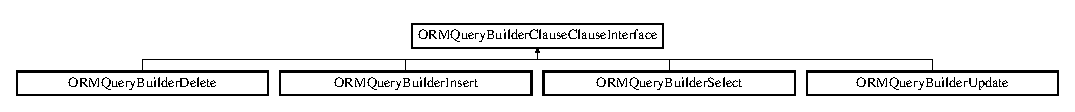
\includegraphics[height=1.056604cm]{interfaceORM_1_1QueryBuilder_1_1Clause_1_1ClauseInterface}
\end{center}
\end{figure}
\subsection*{Public Member Functions}
\begin{DoxyCompactItemize}
\item 
{\bfseries to\+Sql} ()\hypertarget{interfaceORM_1_1QueryBuilder_1_1Clause_1_1ClauseInterface_aa0c6ef99a5eb0f0abd951a796fb391c5}{}\label{interfaceORM_1_1QueryBuilder_1_1Clause_1_1ClauseInterface_aa0c6ef99a5eb0f0abd951a796fb391c5}

\end{DoxyCompactItemize}


The documentation for this interface was generated from the following file\+:\begin{DoxyCompactItemize}
\item 
app/orm/src/\+Query\+Builder/\+Clause/Clause\+Interface.\+php\end{DoxyCompactItemize}

\hypertarget{classORM_1_1Connection}{}\section{O\+RM\textbackslash{}Connection Class Reference}
\label{classORM_1_1Connection}\index{O\+R\+M\textbackslash{}\+Connection@{O\+R\+M\textbackslash{}\+Connection}}
\subsection*{Public Member Functions}
\begin{DoxyCompactItemize}
\item 
{\bfseries \+\_\+\+\_\+construct} (\$host, \$database, \$username, \$password)\hypertarget{classORM_1_1Connection_a1c6ec23c8fbb434230c4eed1d00b70ca}{}\label{classORM_1_1Connection_a1c6ec23c8fbb434230c4eed1d00b70ca}

\end{DoxyCompactItemize}
\subsection*{Static Public Member Functions}
\begin{DoxyCompactItemize}
\item 
static {\bfseries get\+Connection} ()\hypertarget{classORM_1_1Connection_a79212f0ac8a8842e3fe64740c10b8975}{}\label{classORM_1_1Connection_a79212f0ac8a8842e3fe64740c10b8975}

\item 
static {\bfseries get\+Database\+Name} ()\hypertarget{classORM_1_1Connection_a6705d29d14c4a87924db9a18b1294eae}{}\label{classORM_1_1Connection_a6705d29d14c4a87924db9a18b1294eae}

\item 
static {\bfseries reset\+Connection} (\$host, \$database, \$username, \$password)\hypertarget{classORM_1_1Connection_aced85c48449dc401c84abf68f38671e8}{}\label{classORM_1_1Connection_aced85c48449dc401c84abf68f38671e8}

\end{DoxyCompactItemize}


The documentation for this class was generated from the following file\+:\begin{DoxyCompactItemize}
\item 
app/orm/src/Connection.\+php\end{DoxyCompactItemize}

\hypertarget{classORM_1_1Console_1_1Console}{}\section{O\+RM\textbackslash{}Console\textbackslash{}Console Class Reference}
\label{classORM_1_1Console_1_1Console}\index{O\+R\+M\textbackslash{}\+Console\textbackslash{}\+Console@{O\+R\+M\textbackslash{}\+Console\textbackslash{}\+Console}}
\subsection*{Public Member Functions}
\begin{DoxyCompactItemize}
\item 
{\bfseries \+\_\+\+\_\+construct} (\$Entity\+Namespace, array \&\$arg)\hypertarget{classORM_1_1Console_1_1Console_aefac843251e8d9896a7438ea33a8546c}{}\label{classORM_1_1Console_1_1Console_aefac843251e8d9896a7438ea33a8546c}

\end{DoxyCompactItemize}


The documentation for this class was generated from the following file\+:\begin{DoxyCompactItemize}
\item 
app/orm/src/\+Console/Console.\+php\end{DoxyCompactItemize}

\hypertarget{classORM_1_1QueryBuilder_1_1Helper_1_1Count}{}\section{O\+RM\textbackslash{}Query\+Builder\textbackslash{}Helper\textbackslash{}Count Class Reference}
\label{classORM_1_1QueryBuilder_1_1Helper_1_1Count}\index{O\+R\+M\textbackslash{}\+Query\+Builder\textbackslash{}\+Helper\textbackslash{}\+Count@{O\+R\+M\textbackslash{}\+Query\+Builder\textbackslash{}\+Helper\textbackslash{}\+Count}}
Inheritance diagram for O\+RM\textbackslash{}Query\+Builder\textbackslash{}Helper\textbackslash{}Count\+:\begin{figure}[H]
\begin{center}
\leavevmode
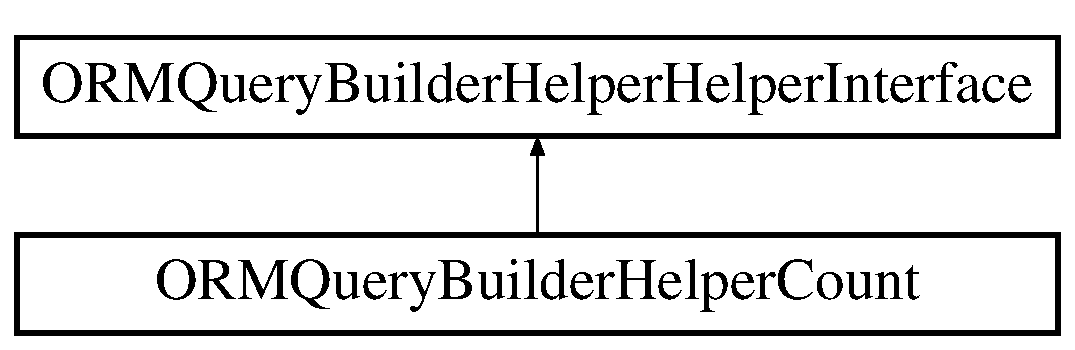
\includegraphics[height=2.000000cm]{classORM_1_1QueryBuilder_1_1Helper_1_1Count}
\end{center}
\end{figure}
\subsection*{Public Member Functions}
\begin{DoxyCompactItemize}
\item 
{\bfseries \+\_\+\+\_\+construct} (\$data)\hypertarget{classORM_1_1QueryBuilder_1_1Helper_1_1Count_a3c620fb9054429d006fa342434b37af9}{}\label{classORM_1_1QueryBuilder_1_1Helper_1_1Count_a3c620fb9054429d006fa342434b37af9}

\item 
{\bfseries get\+Return} ()\hypertarget{classORM_1_1QueryBuilder_1_1Helper_1_1Count_acd979008fc85b69eb1d1a97ad7bb2b3f}{}\label{classORM_1_1QueryBuilder_1_1Helper_1_1Count_acd979008fc85b69eb1d1a97ad7bb2b3f}

\end{DoxyCompactItemize}


The documentation for this class was generated from the following file\+:\begin{DoxyCompactItemize}
\item 
app/orm/src/\+Query\+Builder/\+Helper/Count.\+php\end{DoxyCompactItemize}

\hypertarget{classORM_1_1QueryBuilder_1_1Delete}{}\section{O\+RM\textbackslash{}Query\+Builder\textbackslash{}Delete Class Reference}
\label{classORM_1_1QueryBuilder_1_1Delete}\index{O\+R\+M\textbackslash{}\+Query\+Builder\textbackslash{}\+Delete@{O\+R\+M\textbackslash{}\+Query\+Builder\textbackslash{}\+Delete}}
Inheritance diagram for O\+RM\textbackslash{}Query\+Builder\textbackslash{}Delete\+:\begin{figure}[H]
\begin{center}
\leavevmode
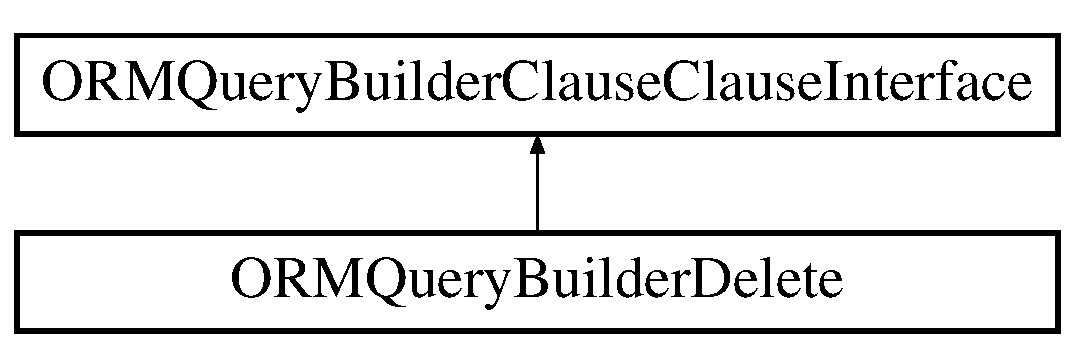
\includegraphics[height=2.000000cm]{classORM_1_1QueryBuilder_1_1Delete}
\end{center}
\end{figure}
\subsection*{Public Member Functions}
\begin{DoxyCompactItemize}
\item 
{\bfseries from} (\$table)\hypertarget{classORM_1_1QueryBuilder_1_1Delete_a63edd9e626091ac44900e3d0b99e78be}{}\label{classORM_1_1QueryBuilder_1_1Delete_a63edd9e626091ac44900e3d0b99e78be}

\item 
{\bfseries to\+Sql} ()\hypertarget{classORM_1_1QueryBuilder_1_1Delete_a775f46779766b6c8360cc1da938116f8}{}\label{classORM_1_1QueryBuilder_1_1Delete_a775f46779766b6c8360cc1da938116f8}

\end{DoxyCompactItemize}


The documentation for this class was generated from the following file\+:\begin{DoxyCompactItemize}
\item 
app/orm/src/\+Query\+Builder/Delete.\+php\end{DoxyCompactItemize}

\hypertarget{classORM_1_1Persistence_1_1DeletePersist}{}\section{O\+RM\textbackslash{}Persistence\textbackslash{}Delete\+Persist Class Reference}
\label{classORM_1_1Persistence_1_1DeletePersist}\index{O\+R\+M\textbackslash{}\+Persistence\textbackslash{}\+Delete\+Persist@{O\+R\+M\textbackslash{}\+Persistence\textbackslash{}\+Delete\+Persist}}
Inheritance diagram for O\+RM\textbackslash{}Persistence\textbackslash{}Delete\+Persist\+:\begin{figure}[H]
\begin{center}
\leavevmode
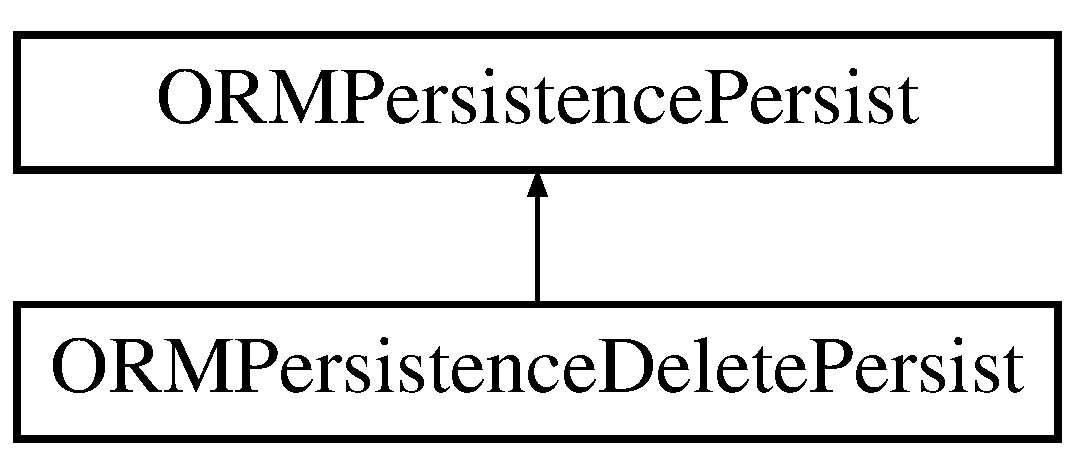
\includegraphics[height=2.000000cm]{classORM_1_1Persistence_1_1DeletePersist}
\end{center}
\end{figure}
\subsection*{Protected Member Functions}
\begin{DoxyCompactItemize}
\item 
{\bfseries analyze} ()\hypertarget{classORM_1_1Persistence_1_1DeletePersist_ac0b22e8b50d88dac861945b437fbaaf9}{}\label{classORM_1_1Persistence_1_1DeletePersist_ac0b22e8b50d88dac861945b437fbaaf9}

\end{DoxyCompactItemize}
\subsection*{Additional Inherited Members}


The documentation for this class was generated from the following file\+:\begin{DoxyCompactItemize}
\item 
app/orm/src/\+Persistence/Delete\+Persist.\+php\end{DoxyCompactItemize}

\hypertarget{classsrc_1_1controller_1_1DemoController}{}\section{src\textbackslash{}controller\textbackslash{}Demo\+Controller Class Reference}
\label{classsrc_1_1controller_1_1DemoController}\index{src\textbackslash{}controller\textbackslash{}\+Demo\+Controller@{src\textbackslash{}controller\textbackslash{}\+Demo\+Controller}}
\subsection*{Public Member Functions}
\begin{DoxyCompactItemize}
\item 
\hyperlink{classsrc_1_1controller_1_1DemoController_ac1c4b80f0fe71221ebcb05c6d632418a}{index} ()
\item 
\hyperlink{classsrc_1_1controller_1_1DemoController_a041b20fb797e78cfe4007e725f804988}{bonjour} ()
\item 
\hyperlink{classsrc_1_1controller_1_1DemoController_a1f001d5a7e9ec53c9241c297220496eb}{argu} (\$args=null)
\item 
\hyperlink{classsrc_1_1controller_1_1DemoController_ab52b0fdd59e32ab14c021af1f5c68434}{tw\+\_\+args} (\$args=N\+U\+LL)
\item 
\hyperlink{classsrc_1_1controller_1_1DemoController_a0772c94750bc03b25505f02a92127956}{orm\+Test} ()
\end{DoxyCompactItemize}


\subsection{Detailed Description}
Class \hyperlink{classsrc_1_1controller_1_1DemoController}{Demo\+Controller} Chemins utilisés pour la démonstration lors de la soutenance du projet 

\subsection{Member Function Documentation}
\index{src\+::controller\+::\+Demo\+Controller@{src\+::controller\+::\+Demo\+Controller}!argu@{argu}}
\index{argu@{argu}!src\+::controller\+::\+Demo\+Controller@{src\+::controller\+::\+Demo\+Controller}}
\subsubsection[{\texorpdfstring{argu(\$args=null)}{argu($args=null)}}]{\setlength{\rightskip}{0pt plus 5cm}src\textbackslash{}controller\textbackslash{}\+Demo\+Controller\+::argu (
\begin{DoxyParamCaption}
\item[{}]{\$args = {\ttfamily null}}
\end{DoxyParamCaption}
)}\hypertarget{classsrc_1_1controller_1_1DemoController_a1f001d5a7e9ec53c9241c297220496eb}{}\label{classsrc_1_1controller_1_1DemoController_a1f001d5a7e9ec53c9241c297220496eb}

\begin{DoxyParams}[1]{Parameters}
null & {\em \$args} & \\
\hline
\end{DoxyParams}
\begin{DoxyReturn}{Returns}
bool Premier test avec retour d\textquotesingle{}arguments \+\_\+\+G\+ET  /test/argu/\{arg\} 
\end{DoxyReturn}
\index{src\+::controller\+::\+Demo\+Controller@{src\+::controller\+::\+Demo\+Controller}!bonjour@{bonjour}}
\index{bonjour@{bonjour}!src\+::controller\+::\+Demo\+Controller@{src\+::controller\+::\+Demo\+Controller}}
\subsubsection[{\texorpdfstring{bonjour()}{bonjour()}}]{\setlength{\rightskip}{0pt plus 5cm}src\textbackslash{}controller\textbackslash{}\+Demo\+Controller\+::bonjour (
\begin{DoxyParamCaption}
{}
\end{DoxyParamCaption}
)}\hypertarget{classsrc_1_1controller_1_1DemoController_a041b20fb797e78cfe4007e725f804988}{}\label{classsrc_1_1controller_1_1DemoController_a041b20fb797e78cfe4007e725f804988}
\begin{DoxyReturn}{Returns}
string Premier test  /test/bonjour 
\end{DoxyReturn}
\index{src\+::controller\+::\+Demo\+Controller@{src\+::controller\+::\+Demo\+Controller}!index@{index}}
\index{index@{index}!src\+::controller\+::\+Demo\+Controller@{src\+::controller\+::\+Demo\+Controller}}
\subsubsection[{\texorpdfstring{index()}{index()}}]{\setlength{\rightskip}{0pt plus 5cm}src\textbackslash{}controller\textbackslash{}\+Demo\+Controller\+::index (
\begin{DoxyParamCaption}
{}
\end{DoxyParamCaption}
)}\hypertarget{classsrc_1_1controller_1_1DemoController_ac1c4b80f0fe71221ebcb05c6d632418a}{}\label{classsrc_1_1controller_1_1DemoController_ac1c4b80f0fe71221ebcb05c6d632418a}
\begin{DoxyReturn}{Returns}
string Page principale à la racine /  / 
\end{DoxyReturn}
\index{src\+::controller\+::\+Demo\+Controller@{src\+::controller\+::\+Demo\+Controller}!orm\+Test@{orm\+Test}}
\index{orm\+Test@{orm\+Test}!src\+::controller\+::\+Demo\+Controller@{src\+::controller\+::\+Demo\+Controller}}
\subsubsection[{\texorpdfstring{orm\+Test()}{ormTest()}}]{\setlength{\rightskip}{0pt plus 5cm}src\textbackslash{}controller\textbackslash{}\+Demo\+Controller\+::orm\+Test (
\begin{DoxyParamCaption}
{}
\end{DoxyParamCaption}
)}\hypertarget{classsrc_1_1controller_1_1DemoController_a0772c94750bc03b25505f02a92127956}{}\label{classsrc_1_1controller_1_1DemoController_a0772c94750bc03b25505f02a92127956}
\begin{DoxyReturn}{Returns}
bool  /orm 
\end{DoxyReturn}
\index{src\+::controller\+::\+Demo\+Controller@{src\+::controller\+::\+Demo\+Controller}!tw\+\_\+args@{tw\+\_\+args}}
\index{tw\+\_\+args@{tw\+\_\+args}!src\+::controller\+::\+Demo\+Controller@{src\+::controller\+::\+Demo\+Controller}}
\subsubsection[{\texorpdfstring{tw\+\_\+args(\$args=\+N\+U\+L\+L)}{tw_args($args=NULL)}}]{\setlength{\rightskip}{0pt plus 5cm}src\textbackslash{}controller\textbackslash{}\+Demo\+Controller\+::tw\+\_\+args (
\begin{DoxyParamCaption}
\item[{}]{\$args = {\ttfamily NULL}}
\end{DoxyParamCaption}
)}\hypertarget{classsrc_1_1controller_1_1DemoController_ab52b0fdd59e32ab14c021af1f5c68434}{}\label{classsrc_1_1controller_1_1DemoController_ab52b0fdd59e32ab14c021af1f5c68434}

\begin{DoxyParams}[1]{Parameters}
null & {\em \$args} & \\
\hline
\end{DoxyParams}
\begin{DoxyReturn}{Returns}
bool Test avec retour d\textquotesingle{}arguments \+\_\+\+G\+ET et affichage Twig  /tw/args/\{arggg\}/\{bien\} 
\end{DoxyReturn}


The documentation for this class was generated from the following file\+:\begin{DoxyCompactItemize}
\item 
src/controller/Demo\+Controller.\+php\end{DoxyCompactItemize}

\hypertarget{classORM_1_1Entity_1_1Entity}{}\section{O\+RM\textbackslash{}Entity\textbackslash{}Entity Class Reference}
\label{classORM_1_1Entity_1_1Entity}\index{O\+R\+M\textbackslash{}\+Entity\textbackslash{}\+Entity@{O\+R\+M\textbackslash{}\+Entity\textbackslash{}\+Entity}}
Inheritance diagram for O\+RM\textbackslash{}Entity\textbackslash{}Entity\+:\begin{figure}[H]
\begin{center}
\leavevmode
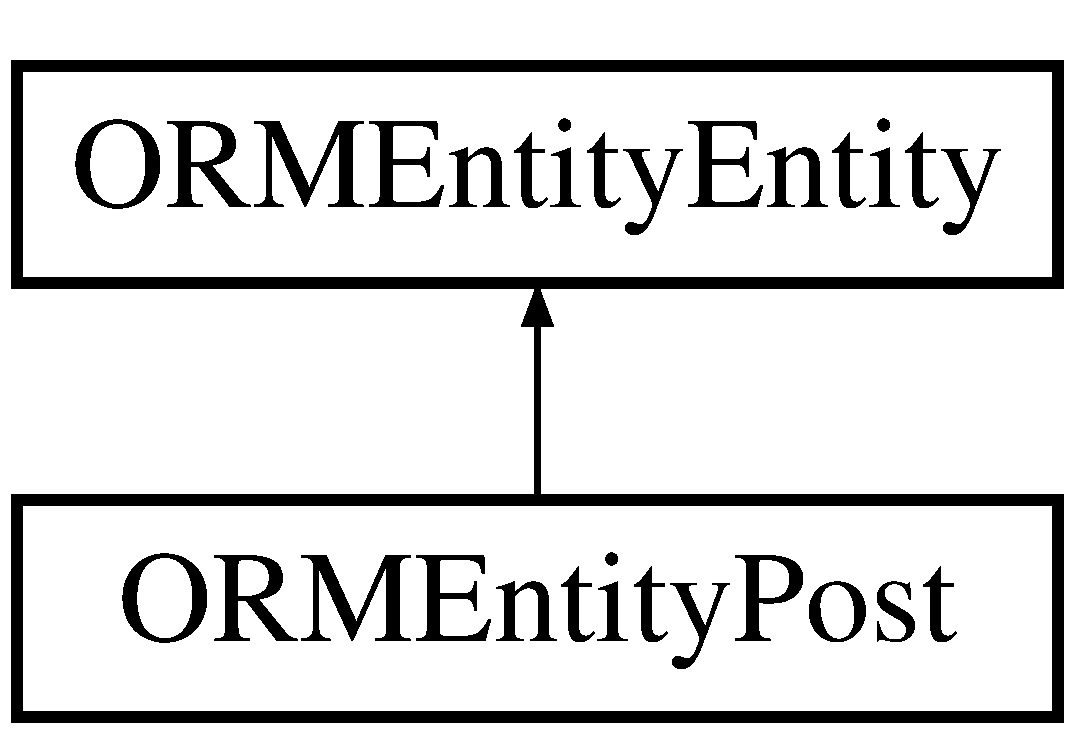
\includegraphics[height=2.000000cm]{classORM_1_1Entity_1_1Entity}
\end{center}
\end{figure}
\subsection*{Public Member Functions}
\begin{DoxyCompactItemize}
\item 
{\bfseries get\+Alias} ()\hypertarget{classORM_1_1Entity_1_1Entity_a6d8eb5967b0478ef2e3d96e7ea940b14}{}\label{classORM_1_1Entity_1_1Entity_a6d8eb5967b0478ef2e3d96e7ea940b14}

\item 
{\bfseries get\+Fields\+Name} ()\hypertarget{classORM_1_1Entity_1_1Entity_ad701973aa9e5faa28e7bc10916405a2b}{}\label{classORM_1_1Entity_1_1Entity_ad701973aa9e5faa28e7bc10916405a2b}

\item 
{\bfseries get\+Fields\+Value} ()\hypertarget{classORM_1_1Entity_1_1Entity_a71eed8c12a7d78c03b4cd0d4d6f60cc5}{}\label{classORM_1_1Entity_1_1Entity_a71eed8c12a7d78c03b4cd0d4d6f60cc5}

\item 
{\bfseries get\+Relation\+Fields} ()\hypertarget{classORM_1_1Entity_1_1Entity_a6391931d6ea29de3080cd262e3b28b9d}{}\label{classORM_1_1Entity_1_1Entity_a6391931d6ea29de3080cd262e3b28b9d}

\item 
{\bfseries has\+Relationship} ()\hypertarget{classORM_1_1Entity_1_1Entity_a7b5e2a8499ab15d609dc3444546f9237}{}\label{classORM_1_1Entity_1_1Entity_a7b5e2a8499ab15d609dc3444546f9237}

\item 
{\bfseries is\+Relationship} (\$field)\hypertarget{classORM_1_1Entity_1_1Entity_ad8388dee9e958896aad552379e495588}{}\label{classORM_1_1Entity_1_1Entity_ad8388dee9e958896aad552379e495588}

\item 
{\bfseries is\+Relationship\+Empty} ()\hypertarget{classORM_1_1Entity_1_1Entity_a2fe2a73ce4726f812fd0e93a8b59020e}{}\label{classORM_1_1Entity_1_1Entity_a2fe2a73ce4726f812fd0e93a8b59020e}

\end{DoxyCompactItemize}
\subsection*{Public Attributes}
\begin{DoxyCompactItemize}
\item 
const {\bfseries E\+X\+P\+L\+O\+D\+E\+\_\+\+C\+H\+AR} = \textquotesingle{}\+\_\+\textquotesingle{}\hypertarget{classORM_1_1Entity_1_1Entity_ad8d1be205ff51b0b7d53a08b0e717f56}{}\label{classORM_1_1Entity_1_1Entity_ad8d1be205ff51b0b7d53a08b0e717f56}

\end{DoxyCompactItemize}


The documentation for this class was generated from the following file\+:\begin{DoxyCompactItemize}
\item 
app/orm/src/\+Entity/Entity.\+php\end{DoxyCompactItemize}

\hypertarget{classORM_1_1Console_1_1Command_1_1Generate_1_1Entity}{}\section{O\+RM\textbackslash{}Console\textbackslash{}Command\textbackslash{}Generate\textbackslash{}Entity Class Reference}
\label{classORM_1_1Console_1_1Command_1_1Generate_1_1Entity}\index{O\+R\+M\textbackslash{}\+Console\textbackslash{}\+Command\textbackslash{}\+Generate\textbackslash{}\+Entity@{O\+R\+M\textbackslash{}\+Console\textbackslash{}\+Command\textbackslash{}\+Generate\textbackslash{}\+Entity}}
\subsection*{Public Member Functions}
\begin{DoxyCompactItemize}
\item 
{\bfseries \+\_\+\+\_\+construct} (\$Entity\+Namespace, \$arg)\hypertarget{classORM_1_1Console_1_1Command_1_1Generate_1_1Entity_a2ffc346999de213700fdf227d3373fa1}{}\label{classORM_1_1Console_1_1Command_1_1Generate_1_1Entity_a2ffc346999de213700fdf227d3373fa1}

\end{DoxyCompactItemize}


The documentation for this class was generated from the following file\+:\begin{DoxyCompactItemize}
\item 
app/orm/src/\+Console/\+Command/\+Generate/Entity.\+php\end{DoxyCompactItemize}

\hypertarget{classORM_1_1Exception_1_1Exception}{}\section{O\+RM\textbackslash{}Exception\textbackslash{}Exception Class Reference}
\label{classORM_1_1Exception_1_1Exception}\index{O\+R\+M\textbackslash{}\+Exception\textbackslash{}\+Exception@{O\+R\+M\textbackslash{}\+Exception\textbackslash{}\+Exception}}
Inheritance diagram for O\+RM\textbackslash{}Exception\textbackslash{}Exception\+:\begin{figure}[H]
\begin{center}
\leavevmode
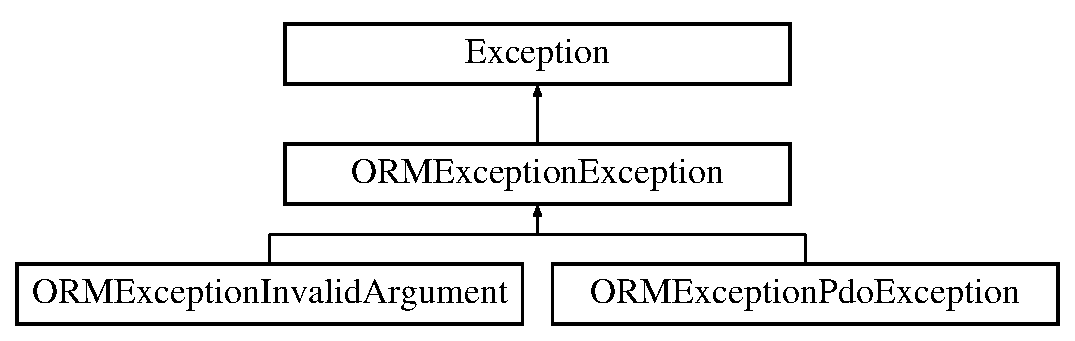
\includegraphics[height=3.000000cm]{classORM_1_1Exception_1_1Exception}
\end{center}
\end{figure}
\subsection*{Public Member Functions}
\begin{DoxyCompactItemize}
\item 
{\bfseries set\+Class\+Name} (\$class\+Name)\hypertarget{classORM_1_1Exception_1_1Exception_a7608581ef97e9ee04fda4001da20206c}{}\label{classORM_1_1Exception_1_1Exception_a7608581ef97e9ee04fda4001da20206c}

\item 
{\bfseries get\+Class\+Name} ()\hypertarget{classORM_1_1Exception_1_1Exception_abffb277c4c2ea6271d26da855263b125}{}\label{classORM_1_1Exception_1_1Exception_abffb277c4c2ea6271d26da855263b125}

\item 
{\bfseries cry} ()\hypertarget{classORM_1_1Exception_1_1Exception_ae620eebdf0ac85cb86421262eb9bab3a}{}\label{classORM_1_1Exception_1_1Exception_ae620eebdf0ac85cb86421262eb9bab3a}

\end{DoxyCompactItemize}
\subsection*{Protected Attributes}
\begin{DoxyCompactItemize}
\item 
{\bfseries \$class\+Name}\hypertarget{classORM_1_1Exception_1_1Exception_a4c9b1310c6b111a2b9add55bffced260}{}\label{classORM_1_1Exception_1_1Exception_a4c9b1310c6b111a2b9add55bffced260}

\end{DoxyCompactItemize}


The documentation for this class was generated from the following file\+:\begin{DoxyCompactItemize}
\item 
app/orm/src/\+Exception/Exception.\+php\end{DoxyCompactItemize}

\hypertarget{classORM_1_1QueryBuilder_1_1Helper_1_1Exist}{}\section{O\+RM\textbackslash{}Query\+Builder\textbackslash{}Helper\textbackslash{}Exist Class Reference}
\label{classORM_1_1QueryBuilder_1_1Helper_1_1Exist}\index{O\+R\+M\textbackslash{}\+Query\+Builder\textbackslash{}\+Helper\textbackslash{}\+Exist@{O\+R\+M\textbackslash{}\+Query\+Builder\textbackslash{}\+Helper\textbackslash{}\+Exist}}
Inheritance diagram for O\+RM\textbackslash{}Query\+Builder\textbackslash{}Helper\textbackslash{}Exist\+:\begin{figure}[H]
\begin{center}
\leavevmode
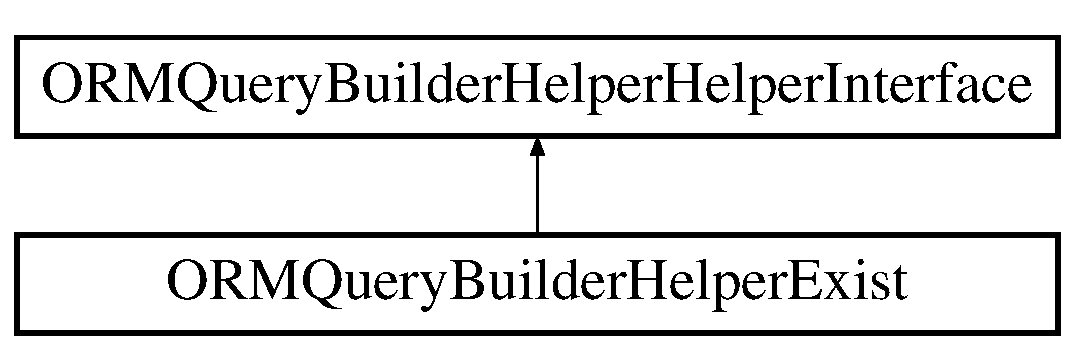
\includegraphics[height=2.000000cm]{classORM_1_1QueryBuilder_1_1Helper_1_1Exist}
\end{center}
\end{figure}
\subsection*{Public Member Functions}
\begin{DoxyCompactItemize}
\item 
{\bfseries \+\_\+\+\_\+construct} (\$data)\hypertarget{classORM_1_1QueryBuilder_1_1Helper_1_1Exist_a839c6c9390d763c00e7187e90347da44}{}\label{classORM_1_1QueryBuilder_1_1Helper_1_1Exist_a839c6c9390d763c00e7187e90347da44}

\item 
{\bfseries get\+Return} ()\hypertarget{classORM_1_1QueryBuilder_1_1Helper_1_1Exist_a4772ad152d497ee7e8c1cf5677ec607d}{}\label{classORM_1_1QueryBuilder_1_1Helper_1_1Exist_a4772ad152d497ee7e8c1cf5677ec607d}

\end{DoxyCompactItemize}


The documentation for this class was generated from the following file\+:\begin{DoxyCompactItemize}
\item 
app/orm/src/\+Query\+Builder/\+Helper/Exist.\+php\end{DoxyCompactItemize}

\hypertarget{interfaceORM_1_1QueryBuilder_1_1Helper_1_1HelperInterface}{}\section{O\+RM\textbackslash{}Query\+Builder\textbackslash{}Helper\textbackslash{}Helper\+Interface Interface Reference}
\label{interfaceORM_1_1QueryBuilder_1_1Helper_1_1HelperInterface}\index{O\+R\+M\textbackslash{}\+Query\+Builder\textbackslash{}\+Helper\textbackslash{}\+Helper\+Interface@{O\+R\+M\textbackslash{}\+Query\+Builder\textbackslash{}\+Helper\textbackslash{}\+Helper\+Interface}}
Inheritance diagram for O\+RM\textbackslash{}Query\+Builder\textbackslash{}Helper\textbackslash{}Helper\+Interface\+:\begin{figure}[H]
\begin{center}
\leavevmode
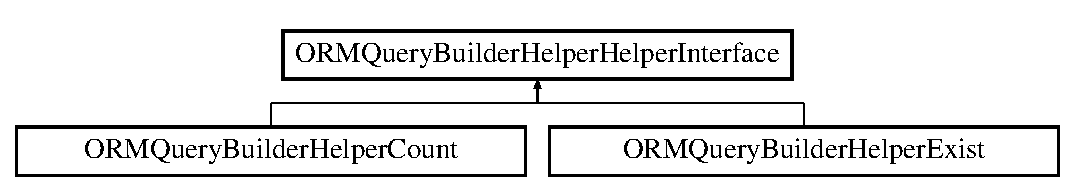
\includegraphics[height=2.000000cm]{interfaceORM_1_1QueryBuilder_1_1Helper_1_1HelperInterface}
\end{center}
\end{figure}
\subsection*{Public Member Functions}
\begin{DoxyCompactItemize}
\item 
{\bfseries \+\_\+\+\_\+construct} (\$data)\hypertarget{interfaceORM_1_1QueryBuilder_1_1Helper_1_1HelperInterface_a4a0602f6a49bbe0feab9b037393c8a59}{}\label{interfaceORM_1_1QueryBuilder_1_1Helper_1_1HelperInterface_a4a0602f6a49bbe0feab9b037393c8a59}

\item 
{\bfseries get\+Return} ()\hypertarget{interfaceORM_1_1QueryBuilder_1_1Helper_1_1HelperInterface_a8dea6a506c7d4209a23370035eb0356a}{}\label{interfaceORM_1_1QueryBuilder_1_1Helper_1_1HelperInterface_a8dea6a506c7d4209a23370035eb0356a}

\end{DoxyCompactItemize}


The documentation for this interface was generated from the following file\+:\begin{DoxyCompactItemize}
\item 
app/orm/src/\+Query\+Builder/\+Helper/Helper\+Interface.\+php\end{DoxyCompactItemize}

\hypertarget{classORM_1_1Entity_1_1Hydrate}{}\section{O\+RM\textbackslash{}Entity\textbackslash{}Hydrate Class Reference}
\label{classORM_1_1Entity_1_1Hydrate}\index{O\+R\+M\textbackslash{}\+Entity\textbackslash{}\+Hydrate@{O\+R\+M\textbackslash{}\+Entity\textbackslash{}\+Hydrate}}
\subsection*{Public Member Functions}
\begin{DoxyCompactItemize}
\item 
{\bfseries set\+Sql\+Result} (\$sql\+\_\+result)\hypertarget{classORM_1_1Entity_1_1Hydrate_a2b37dc9f3af5c1538a1ee6f0b6291c68}{}\label{classORM_1_1Entity_1_1Hydrate_a2b37dc9f3af5c1538a1ee6f0b6291c68}

\item 
{\bfseries get\+Sql\+Result} ()\hypertarget{classORM_1_1Entity_1_1Hydrate_a083c239d6782e20815b7822082e18089}{}\label{classORM_1_1Entity_1_1Hydrate_a083c239d6782e20815b7822082e18089}

\item 
{\bfseries hydrate} ()\hypertarget{classORM_1_1Entity_1_1Hydrate_a24446d2308e8ca1ef2ab0eaaf5945e75}{}\label{classORM_1_1Entity_1_1Hydrate_a24446d2308e8ca1ef2ab0eaaf5945e75}

\end{DoxyCompactItemize}


The documentation for this class was generated from the following file\+:\begin{DoxyCompactItemize}
\item 
app/orm/src/\+Entity/Hydrate.\+php\end{DoxyCompactItemize}

\hypertarget{classORM_1_1QueryBuilder_1_1Insert}{}\section{O\+RM\textbackslash{}Query\+Builder\textbackslash{}Insert Class Reference}
\label{classORM_1_1QueryBuilder_1_1Insert}\index{O\+R\+M\textbackslash{}\+Query\+Builder\textbackslash{}\+Insert@{O\+R\+M\textbackslash{}\+Query\+Builder\textbackslash{}\+Insert}}
Inheritance diagram for O\+RM\textbackslash{}Query\+Builder\textbackslash{}Insert\+:\begin{figure}[H]
\begin{center}
\leavevmode
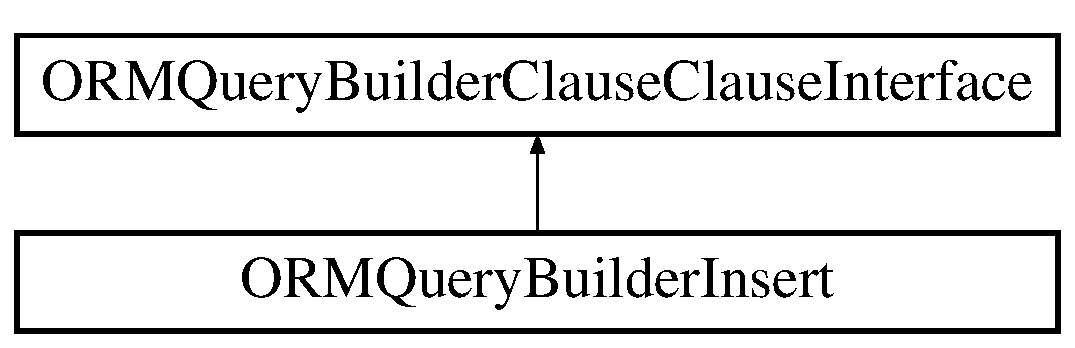
\includegraphics[height=2.000000cm]{classORM_1_1QueryBuilder_1_1Insert}
\end{center}
\end{figure}
\subsection*{Public Member Functions}
\begin{DoxyCompactItemize}
\item 
{\bfseries into} (\$table, \$values=false)\hypertarget{classORM_1_1QueryBuilder_1_1Insert_a6f3684a358d8d95f4875a0bb339ae373}{}\label{classORM_1_1QueryBuilder_1_1Insert_a6f3684a358d8d95f4875a0bb339ae373}

\item 
{\bfseries values} (\$values)\hypertarget{classORM_1_1QueryBuilder_1_1Insert_aeaa8cf2d5d69755eba9999a8d3e42e6e}{}\label{classORM_1_1QueryBuilder_1_1Insert_aeaa8cf2d5d69755eba9999a8d3e42e6e}

\item 
{\bfseries to\+Sql} ()\hypertarget{classORM_1_1QueryBuilder_1_1Insert_ab72e936fbe94621967aa440f6077ae67}{}\label{classORM_1_1QueryBuilder_1_1Insert_ab72e936fbe94621967aa440f6077ae67}

\end{DoxyCompactItemize}


The documentation for this class was generated from the following file\+:\begin{DoxyCompactItemize}
\item 
app/orm/src/\+Query\+Builder/Insert.\+php\end{DoxyCompactItemize}

\hypertarget{classORM_1_1Persistence_1_1InsertPersist}{}\section{O\+RM\textbackslash{}Persistence\textbackslash{}Insert\+Persist Class Reference}
\label{classORM_1_1Persistence_1_1InsertPersist}\index{O\+R\+M\textbackslash{}\+Persistence\textbackslash{}\+Insert\+Persist@{O\+R\+M\textbackslash{}\+Persistence\textbackslash{}\+Insert\+Persist}}
Inheritance diagram for O\+RM\textbackslash{}Persistence\textbackslash{}Insert\+Persist\+:\begin{figure}[H]
\begin{center}
\leavevmode
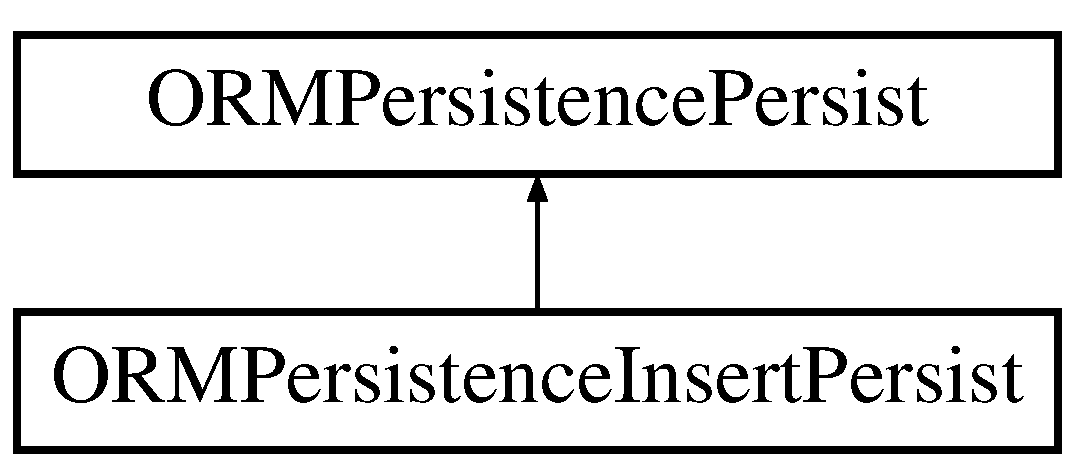
\includegraphics[height=2.000000cm]{classORM_1_1Persistence_1_1InsertPersist}
\end{center}
\end{figure}
\subsection*{Protected Member Functions}
\begin{DoxyCompactItemize}
\item 
{\bfseries analyze} ()\hypertarget{classORM_1_1Persistence_1_1InsertPersist_a6a9673546ee81a4d6998c501a030b359}{}\label{classORM_1_1Persistence_1_1InsertPersist_a6a9673546ee81a4d6998c501a030b359}

\end{DoxyCompactItemize}
\subsection*{Additional Inherited Members}


The documentation for this class was generated from the following file\+:\begin{DoxyCompactItemize}
\item 
app/orm/src/\+Persistence/Insert\+Persist.\+php\end{DoxyCompactItemize}

\hypertarget{classORM_1_1Exception_1_1InvalidArgument}{}\section{O\+RM\textbackslash{}Exception\textbackslash{}Invalid\+Argument Class Reference}
\label{classORM_1_1Exception_1_1InvalidArgument}\index{O\+R\+M\textbackslash{}\+Exception\textbackslash{}\+Invalid\+Argument@{O\+R\+M\textbackslash{}\+Exception\textbackslash{}\+Invalid\+Argument}}
Inheritance diagram for O\+RM\textbackslash{}Exception\textbackslash{}Invalid\+Argument\+:\begin{figure}[H]
\begin{center}
\leavevmode
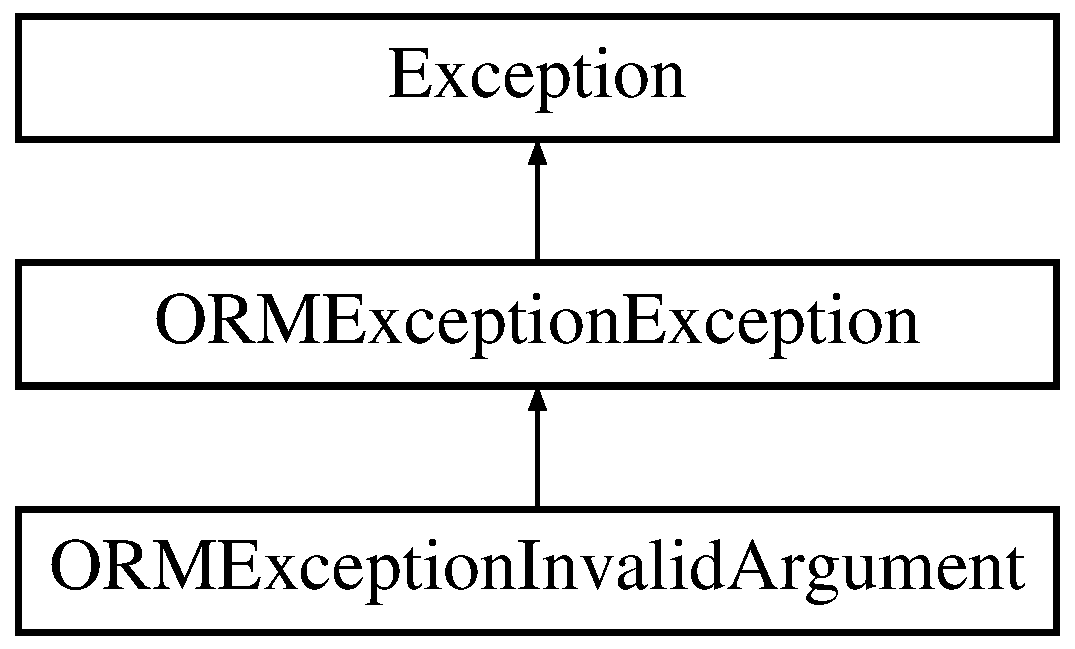
\includegraphics[height=3.000000cm]{classORM_1_1Exception_1_1InvalidArgument}
\end{center}
\end{figure}
\subsection*{Additional Inherited Members}


The documentation for this class was generated from the following file\+:\begin{DoxyCompactItemize}
\item 
app/orm/src/\+Exception/Invalid\+Argument.\+php\end{DoxyCompactItemize}

\hypertarget{classORM_1_1Tools_1_1Logger}{}\section{O\+RM\textbackslash{}Tools\textbackslash{}Logger Class Reference}
\label{classORM_1_1Tools_1_1Logger}\index{O\+R\+M\textbackslash{}\+Tools\textbackslash{}\+Logger@{O\+R\+M\textbackslash{}\+Tools\textbackslash{}\+Logger}}
\subsection*{Public Member Functions}
\begin{DoxyCompactItemize}
\item 
{\bfseries \+\_\+\+\_\+construct} (\$file)\hypertarget{classORM_1_1Tools_1_1Logger_aec350111b1a1558fc901226051b26ac7}{}\label{classORM_1_1Tools_1_1Logger_aec350111b1a1558fc901226051b26ac7}

\item 
{\bfseries add} (\$string)\hypertarget{classORM_1_1Tools_1_1Logger_ab25c5234787b2bb913ed62a7f5ea8a2d}{}\label{classORM_1_1Tools_1_1Logger_ab25c5234787b2bb913ed62a7f5ea8a2d}

\end{DoxyCompactItemize}


The documentation for this class was generated from the following file\+:\begin{DoxyCompactItemize}
\item 
app/orm/src/\+Tools/Logger.\+php\end{DoxyCompactItemize}

\hypertarget{classORM_1_1Entity_1_1Manager}{}\section{O\+RM\textbackslash{}Entity\textbackslash{}Manager Class Reference}
\label{classORM_1_1Entity_1_1Manager}\index{O\+R\+M\textbackslash{}\+Entity\textbackslash{}\+Manager@{O\+R\+M\textbackslash{}\+Entity\textbackslash{}\+Manager}}
\subsection*{Public Member Functions}
\begin{DoxyCompactItemize}
\item 
{\bfseries get\+Repository} (\$\hyperlink{classORM_1_1Entity_1_1Entity}{Entity})\hypertarget{classORM_1_1Entity_1_1Manager_a4cbbaa3a1d3ee9618250ce0c293bba0d}{}\label{classORM_1_1Entity_1_1Manager_a4cbbaa3a1d3ee9618250ce0c293bba0d}

\item 
{\bfseries persist} (\hyperlink{classORM_1_1Entity_1_1Entity}{Entity} \&\$\hyperlink{classORM_1_1Entity_1_1Entity}{Entity})\hypertarget{classORM_1_1Entity_1_1Manager_a03fa49bbe3d431c71432a21634707d19}{}\label{classORM_1_1Entity_1_1Manager_a03fa49bbe3d431c71432a21634707d19}

\item 
{\bfseries remove} (\hyperlink{classORM_1_1Entity_1_1Entity}{Entity} \&\$\hyperlink{classORM_1_1Entity_1_1Entity}{Entity})\hypertarget{classORM_1_1Entity_1_1Manager_a982ca1c24366de2fe472258f4d0d9ae7}{}\label{classORM_1_1Entity_1_1Manager_a982ca1c24366de2fe472258f4d0d9ae7}

\end{DoxyCompactItemize}


The documentation for this class was generated from the following file\+:\begin{DoxyCompactItemize}
\item 
app/orm/src/\+Entity/Manager.\+php\end{DoxyCompactItemize}

\hypertarget{classORM_1_1Entity_1_1Mapping_1_1ManyToOne}{}\section{O\+RM\textbackslash{}Entity\textbackslash{}Mapping\textbackslash{}Many\+To\+One Class Reference}
\label{classORM_1_1Entity_1_1Mapping_1_1ManyToOne}\index{O\+R\+M\textbackslash{}\+Entity\textbackslash{}\+Mapping\textbackslash{}\+Many\+To\+One@{O\+R\+M\textbackslash{}\+Entity\textbackslash{}\+Mapping\textbackslash{}\+Many\+To\+One}}
\subsection*{Public Member Functions}
\begin{DoxyCompactItemize}
\item 
{\bfseries \+\_\+\+\_\+construct} (\&\$\hyperlink{classORM_1_1Entity_1_1Entity}{Entity}, \$relation\+Entity)\hypertarget{classORM_1_1Entity_1_1Mapping_1_1ManyToOne_af74e5bd7db3206cd1ee6db1c2b15e66c}{}\label{classORM_1_1Entity_1_1Mapping_1_1ManyToOne_af74e5bd7db3206cd1ee6db1c2b15e66c}

\item 
{\bfseries get\+Entity} ()\hypertarget{classORM_1_1Entity_1_1Mapping_1_1ManyToOne_ad665ef90a1a8564723d6d6ad75b1ad33}{}\label{classORM_1_1Entity_1_1Mapping_1_1ManyToOne_ad665ef90a1a8564723d6d6ad75b1ad33}

\item 
{\bfseries get\+New\+Relation\+Entity} ()\hypertarget{classORM_1_1Entity_1_1Mapping_1_1ManyToOne_aa5a67b9244dd29bb095013c0aa5090c9}{}\label{classORM_1_1Entity_1_1Mapping_1_1ManyToOne_aa5a67b9244dd29bb095013c0aa5090c9}

\item 
{\bfseries set} (\$\hyperlink{classORM_1_1Entity_1_1Entity}{Entity})\hypertarget{classORM_1_1Entity_1_1Mapping_1_1ManyToOne_af3cad036354899307d6b0d3dc6ea943d}{}\label{classORM_1_1Entity_1_1Mapping_1_1ManyToOne_af3cad036354899307d6b0d3dc6ea943d}

\item 
{\bfseries get} ()\hypertarget{classORM_1_1Entity_1_1Mapping_1_1ManyToOne_a00f86301298aa86567c5b99032748f64}{}\label{classORM_1_1Entity_1_1Mapping_1_1ManyToOne_a00f86301298aa86567c5b99032748f64}

\item 
{\bfseries is\+Empty} ()\hypertarget{classORM_1_1Entity_1_1Mapping_1_1ManyToOne_a6c12f9ea6517afc325632f1c132c3d17}{}\label{classORM_1_1Entity_1_1Mapping_1_1ManyToOne_a6c12f9ea6517afc325632f1c132c3d17}

\end{DoxyCompactItemize}
\subsection*{Public Attributes}
\begin{DoxyCompactItemize}
\item 
const {\bfseries R\+E\+L\+A\+T\+I\+O\+N\+\_\+\+T\+Y\+PE} = \textquotesingle{}\hyperlink{classORM_1_1Entity_1_1Mapping_1_1ManyToOne}{Many\+To\+One}\textquotesingle{}\hypertarget{classORM_1_1Entity_1_1Mapping_1_1ManyToOne_a01ce13e9e2e768ab3b6e33ce8a71dd32}{}\label{classORM_1_1Entity_1_1Mapping_1_1ManyToOne_a01ce13e9e2e768ab3b6e33ce8a71dd32}

\end{DoxyCompactItemize}


The documentation for this class was generated from the following file\+:\begin{DoxyCompactItemize}
\item 
app/orm/src/\+Entity/\+Mapping/Many\+To\+One.\+php\end{DoxyCompactItemize}

\hypertarget{classOrmController}{}\section{Orm\+Controller Class Reference}
\label{classOrmController}\index{Orm\+Controller@{Orm\+Controller}}
\subsection*{Public Member Functions}
\begin{DoxyCompactItemize}
\item 
\hyperlink{classOrmController_a2c7c36a2d2ed060cc77eca678e75ab54}{orm\+Test} ()
\end{DoxyCompactItemize}


\subsection{Detailed Description}
Class \hyperlink{classOrmController}{Orm\+Controller} Second controller pour le test de l\textquotesingle{}\hyperlink{namespaceORM}{O\+RM} 

\subsection{Member Function Documentation}
\index{Orm\+Controller@{Orm\+Controller}!orm\+Test@{orm\+Test}}
\index{orm\+Test@{orm\+Test}!Orm\+Controller@{Orm\+Controller}}
\subsubsection[{\texorpdfstring{orm\+Test()}{ormTest()}}]{\setlength{\rightskip}{0pt plus 5cm}Orm\+Controller\+::orm\+Test (
\begin{DoxyParamCaption}
{}
\end{DoxyParamCaption}
)}\hypertarget{classOrmController_a2c7c36a2d2ed060cc77eca678e75ab54}{}\label{classOrmController_a2c7c36a2d2ed060cc77eca678e75ab54}
\begin{DoxyReturn}{Returns}
bool  /orm 
\end{DoxyReturn}


The documentation for this class was generated from the following file\+:\begin{DoxyCompactItemize}
\item 
src/controller/Orm\+Controller.\+php\end{DoxyCompactItemize}

\hypertarget{classORM_1_1Exception_1_1PdoException}{}\section{O\+RM\textbackslash{}Exception\textbackslash{}Pdo\+Exception Class Reference}
\label{classORM_1_1Exception_1_1PdoException}\index{O\+R\+M\textbackslash{}\+Exception\textbackslash{}\+Pdo\+Exception@{O\+R\+M\textbackslash{}\+Exception\textbackslash{}\+Pdo\+Exception}}
Inheritance diagram for O\+RM\textbackslash{}Exception\textbackslash{}Pdo\+Exception\+:\begin{figure}[H]
\begin{center}
\leavevmode
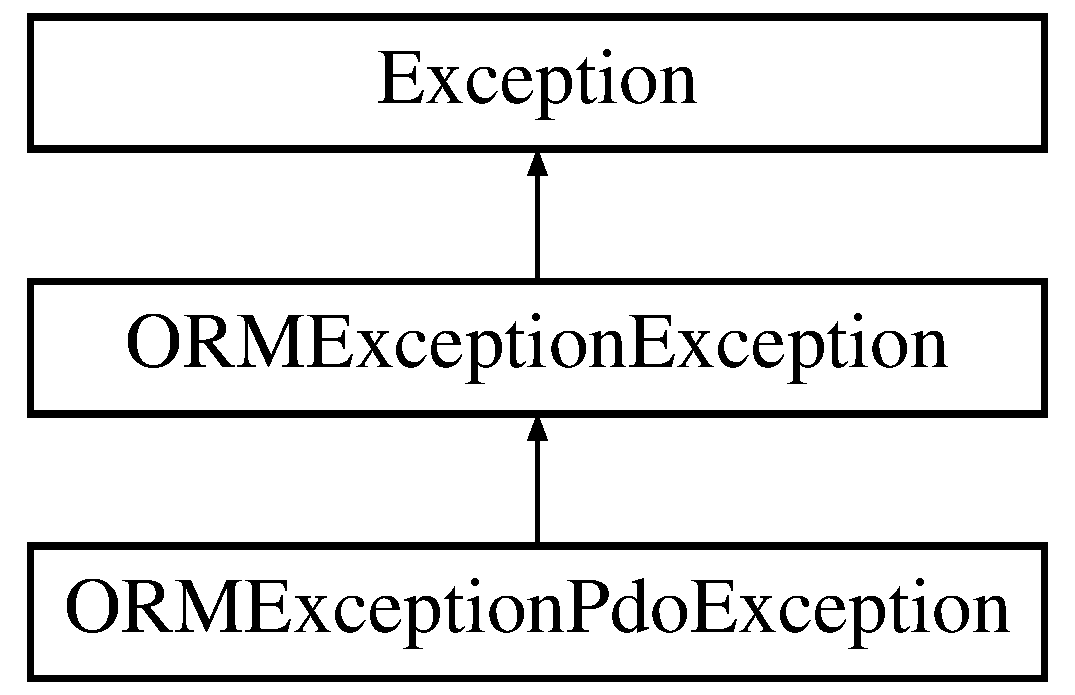
\includegraphics[height=3.000000cm]{classORM_1_1Exception_1_1PdoException}
\end{center}
\end{figure}
\subsection*{Additional Inherited Members}


The documentation for this class was generated from the following file\+:\begin{DoxyCompactItemize}
\item 
app/orm/src/\+Exception/Pdo\+Exception.\+php\end{DoxyCompactItemize}

\hypertarget{classORM_1_1Persistence_1_1Persist}{}\section{O\+RM\textbackslash{}Persistence\textbackslash{}Persist Class Reference}
\label{classORM_1_1Persistence_1_1Persist}\index{O\+R\+M\textbackslash{}\+Persistence\textbackslash{}\+Persist@{O\+R\+M\textbackslash{}\+Persistence\textbackslash{}\+Persist}}
Inheritance diagram for O\+RM\textbackslash{}Persistence\textbackslash{}Persist\+:\begin{figure}[H]
\begin{center}
\leavevmode
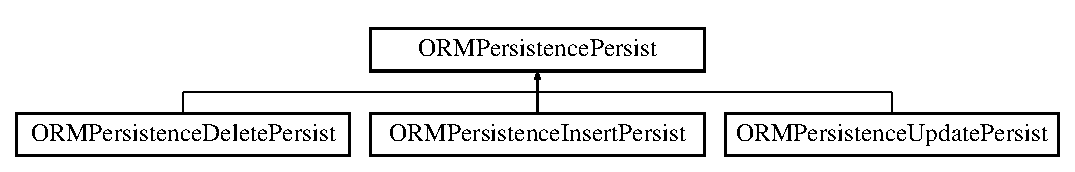
\includegraphics[height=1.866667cm]{classORM_1_1Persistence_1_1Persist}
\end{center}
\end{figure}
\subsection*{Public Member Functions}
\begin{DoxyCompactItemize}
\item 
{\bfseries \+\_\+\+\_\+construct} (\&\$Entity)\hypertarget{classORM_1_1Persistence_1_1Persist_a9d8f1baeb95f36d4af14265a34d9c54a}{}\label{classORM_1_1Persistence_1_1Persist_a9d8f1baeb95f36d4af14265a34d9c54a}

\end{DoxyCompactItemize}
\subsection*{Static Public Member Functions}
\begin{DoxyCompactItemize}
\item 
static {\bfseries check\+Persistence\+Type} (\&\$Entity, \$delete=false)\hypertarget{classORM_1_1Persistence_1_1Persist_ab5871bff08c819c24621ad32ed89ef55}{}\label{classORM_1_1Persistence_1_1Persist_ab5871bff08c819c24621ad32ed89ef55}

\end{DoxyCompactItemize}
\subsection*{Protected Member Functions}
\begin{DoxyCompactItemize}
\item 
{\bfseries persist} (\$array=\mbox{[}$\,$\mbox{]})\hypertarget{classORM_1_1Persistence_1_1Persist_ab1681a85d3a2031c0beb1a2908067c3b}{}\label{classORM_1_1Persistence_1_1Persist_ab1681a85d3a2031c0beb1a2908067c3b}

\item 
{\bfseries analyze} ()\hypertarget{classORM_1_1Persistence_1_1Persist_acb5ee239c02a21c6f25d05fc0786a8d7}{}\label{classORM_1_1Persistence_1_1Persist_acb5ee239c02a21c6f25d05fc0786a8d7}

\item 
{\bfseries get\+Entity} ()\hypertarget{classORM_1_1Persistence_1_1Persist_ac21a3c6871afbd04e0a246de8d0a7454}{}\label{classORM_1_1Persistence_1_1Persist_ac21a3c6871afbd04e0a246de8d0a7454}

\end{DoxyCompactItemize}
\subsection*{Protected Attributes}
\begin{DoxyCompactItemize}
\item 
{\bfseries \$\+Entity}\hypertarget{classORM_1_1Persistence_1_1Persist_a01fde0f4d76bab25e8352f5edbd5fb4d}{}\label{classORM_1_1Persistence_1_1Persist_a01fde0f4d76bab25e8352f5edbd5fb4d}

\item 
{\bfseries \$las\+Id}\hypertarget{classORM_1_1Persistence_1_1Persist_a71f64da053ccb7f7b3b09e67ffbb6678}{}\label{classORM_1_1Persistence_1_1Persist_a71f64da053ccb7f7b3b09e67ffbb6678}

\end{DoxyCompactItemize}


The documentation for this class was generated from the following file\+:\begin{DoxyCompactItemize}
\item 
app/orm/src/\+Persistence/Persist.\+php\end{DoxyCompactItemize}

\hypertarget{classORM_1_1Entity_1_1Post}{}\section{O\+RM\textbackslash{}Entity\textbackslash{}Post Class Reference}
\label{classORM_1_1Entity_1_1Post}\index{O\+R\+M\textbackslash{}\+Entity\textbackslash{}\+Post@{O\+R\+M\textbackslash{}\+Entity\textbackslash{}\+Post}}
Inheritance diagram for O\+RM\textbackslash{}Entity\textbackslash{}Post\+:\begin{figure}[H]
\begin{center}
\leavevmode
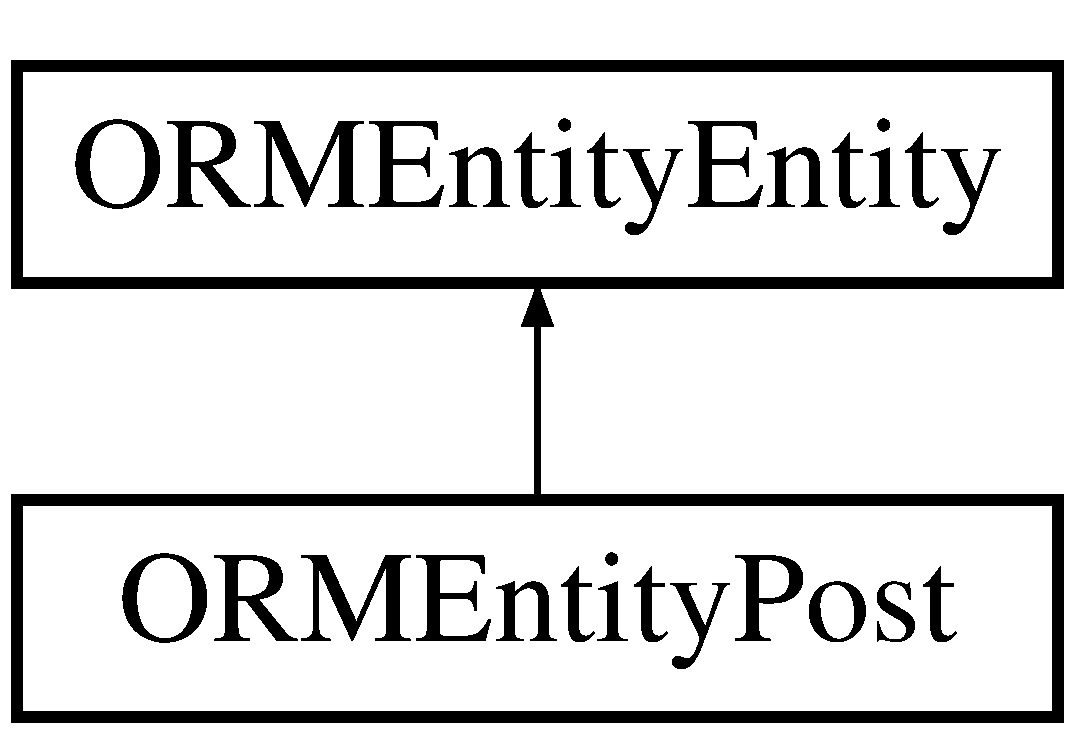
\includegraphics[height=2.000000cm]{classORM_1_1Entity_1_1Post}
\end{center}
\end{figure}
\subsection*{Public Member Functions}
\begin{DoxyCompactItemize}
\item 
{\bfseries set\+Id} (\$id)\hypertarget{classORM_1_1Entity_1_1Post_aac5ab59a4b73b107e5acdae2ec4bf9f5}{}\label{classORM_1_1Entity_1_1Post_aac5ab59a4b73b107e5acdae2ec4bf9f5}

\item 
{\bfseries get\+Id} ()\hypertarget{classORM_1_1Entity_1_1Post_af28422f77735e94d200c12ff9bf4b45b}{}\label{classORM_1_1Entity_1_1Post_af28422f77735e94d200c12ff9bf4b45b}

\item 
{\bfseries set\+Title} (\$title)\hypertarget{classORM_1_1Entity_1_1Post_a5fc1167b1cd76d355ddd0d0828379b34}{}\label{classORM_1_1Entity_1_1Post_a5fc1167b1cd76d355ddd0d0828379b34}

\item 
{\bfseries get\+Title} ()\hypertarget{classORM_1_1Entity_1_1Post_a9e149fe1680157db50a8937be4395610}{}\label{classORM_1_1Entity_1_1Post_a9e149fe1680157db50a8937be4395610}

\item 
{\bfseries set\+Content} (\$content)\hypertarget{classORM_1_1Entity_1_1Post_aa170fe8b65c57e6b75e966f72c33c6de}{}\label{classORM_1_1Entity_1_1Post_aa170fe8b65c57e6b75e966f72c33c6de}

\item 
{\bfseries get\+Content} ()\hypertarget{classORM_1_1Entity_1_1Post_a208c2b207ee804515f26512edb9edab8}{}\label{classORM_1_1Entity_1_1Post_a208c2b207ee804515f26512edb9edab8}

\end{DoxyCompactItemize}
\subsection*{Public Attributes}
\begin{DoxyCompactItemize}
\item 
const {\bfseries T\+A\+B\+LE} = \textquotesingle{}post\textquotesingle{}\hypertarget{classORM_1_1Entity_1_1Post_af42a28989e17709a08106c57b6cb2f4c}{}\label{classORM_1_1Entity_1_1Post_af42a28989e17709a08106c57b6cb2f4c}

\end{DoxyCompactItemize}
\subsection*{Protected Attributes}
\begin{DoxyCompactItemize}
\item 
{\bfseries \$id}\hypertarget{classORM_1_1Entity_1_1Post_af60076c67953553bac9cde5a24247892}{}\label{classORM_1_1Entity_1_1Post_af60076c67953553bac9cde5a24247892}

\item 
{\bfseries \$title}\hypertarget{classORM_1_1Entity_1_1Post_a97fcb96648ad219d0e928b6545fe28bb}{}\label{classORM_1_1Entity_1_1Post_a97fcb96648ad219d0e928b6545fe28bb}

\item 
{\bfseries \$content}\hypertarget{classORM_1_1Entity_1_1Post_a1846e68b722e1abc0d18c79d1dfeb53f}{}\label{classORM_1_1Entity_1_1Post_a1846e68b722e1abc0d18c79d1dfeb53f}

\end{DoxyCompactItemize}


The documentation for this class was generated from the following file\+:\begin{DoxyCompactItemize}
\item 
app/orm/src/\+Entity/Post.\+php\end{DoxyCompactItemize}

\hypertarget{classORM_1_1QueryBuilder_1_1QueryBuilder}{}\section{O\+RM\textbackslash{}Query\+Builder\textbackslash{}Query\+Builder Class Reference}
\label{classORM_1_1QueryBuilder_1_1QueryBuilder}\index{O\+R\+M\textbackslash{}\+Query\+Builder\textbackslash{}\+Query\+Builder@{O\+R\+M\textbackslash{}\+Query\+Builder\textbackslash{}\+Query\+Builder}}
\subsection*{Static Public Member Functions}
\begin{DoxyCompactItemize}
\item 
static {\bfseries execute} (array \$array=\mbox{[}$\,$\mbox{]})\hypertarget{classORM_1_1QueryBuilder_1_1QueryBuilder_a04b38cded552e8b70c48f0e54c6d56ca}{}\label{classORM_1_1QueryBuilder_1_1QueryBuilder_a04b38cded552e8b70c48f0e54c6d56ca}

\item 
static {\bfseries query} (\$sql, \$params=\mbox{[}$\,$\mbox{]})\hypertarget{classORM_1_1QueryBuilder_1_1QueryBuilder_aa61da745454f5038bb6f7786673ef2b8}{}\label{classORM_1_1QueryBuilder_1_1QueryBuilder_aa61da745454f5038bb6f7786673ef2b8}

\end{DoxyCompactItemize}


The documentation for this class was generated from the following file\+:\begin{DoxyCompactItemize}
\item 
app/orm/src/\+Query\+Builder/Query\+Builder.\+php\end{DoxyCompactItemize}

\hypertarget{classORM_1_1Entity_1_1Repository}{}\section{O\+RM\textbackslash{}Entity\textbackslash{}Repository Class Reference}
\label{classORM_1_1Entity_1_1Repository}\index{O\+R\+M\textbackslash{}\+Entity\textbackslash{}\+Repository@{O\+R\+M\textbackslash{}\+Entity\textbackslash{}\+Repository}}
\subsection*{Public Member Functions}
\begin{DoxyCompactItemize}
\item 
{\bfseries \+\_\+\+\_\+construct} (\hyperlink{classORM_1_1Entity_1_1Entity}{Entity} \$\hyperlink{classORM_1_1Entity_1_1Entity}{Entity})\hypertarget{classORM_1_1Entity_1_1Repository_a3e472496199770de24159c9309894d2b}{}\label{classORM_1_1Entity_1_1Repository_a3e472496199770de24159c9309894d2b}

\item 
{\bfseries find\+All} (\$params=\mbox{[}$\,$\mbox{]})\hypertarget{classORM_1_1Entity_1_1Repository_aeabca11d0cfa0b1fa69056dc2d614915}{}\label{classORM_1_1Entity_1_1Repository_aeabca11d0cfa0b1fa69056dc2d614915}

\end{DoxyCompactItemize}
\subsection*{Protected Attributes}
\begin{DoxyCompactItemize}
\item 
{\bfseries \$\+Entity}\hypertarget{classORM_1_1Entity_1_1Repository_a3b30ae1a5be87911bc7f7bafa8f37af5}{}\label{classORM_1_1Entity_1_1Repository_a3b30ae1a5be87911bc7f7bafa8f37af5}

\end{DoxyCompactItemize}


The documentation for this class was generated from the following file\+:\begin{DoxyCompactItemize}
\item 
app/orm/src/\+Entity/Repository.\+php\end{DoxyCompactItemize}

\hypertarget{classcore_1_1Router}{}\section{core\textbackslash{}Router Class Reference}
\label{classcore_1_1Router}\index{core\textbackslash{}\+Router@{core\textbackslash{}\+Router}}
\subsection*{Public Member Functions}
\begin{DoxyCompactItemize}
\item 
{\bfseries run} (\$route)\hypertarget{classcore_1_1Router_a851f70282c4ad784a3ea04c643860969}{}\label{classcore_1_1Router_a851f70282c4ad784a3ea04c643860969}

\end{DoxyCompactItemize}


The documentation for this class was generated from the following file\+:\begin{DoxyCompactItemize}
\item 
core/Router.\+php\end{DoxyCompactItemize}

\hypertarget{classORM_1_1QueryBuilder_1_1Select}{}\section{O\+RM\textbackslash{}Query\+Builder\textbackslash{}Select Class Reference}
\label{classORM_1_1QueryBuilder_1_1Select}\index{O\+R\+M\textbackslash{}\+Query\+Builder\textbackslash{}\+Select@{O\+R\+M\textbackslash{}\+Query\+Builder\textbackslash{}\+Select}}
Inheritance diagram for O\+RM\textbackslash{}Query\+Builder\textbackslash{}Select\+:\begin{figure}[H]
\begin{center}
\leavevmode
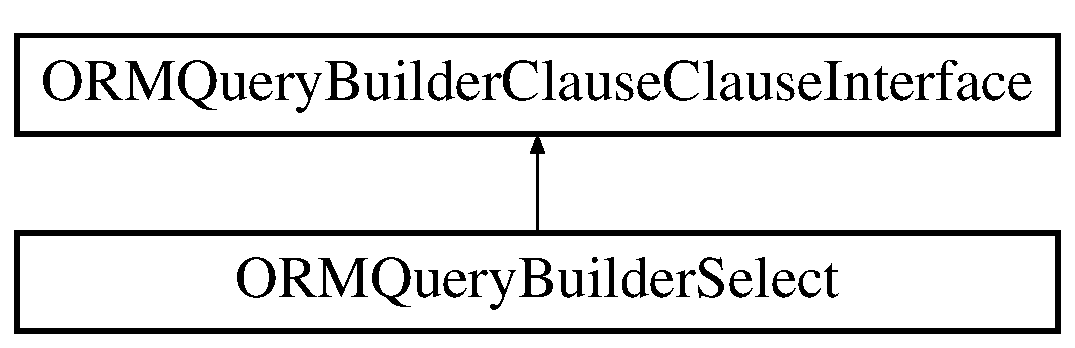
\includegraphics[height=2.000000cm]{classORM_1_1QueryBuilder_1_1Select}
\end{center}
\end{figure}
\subsection*{Public Member Functions}
\begin{DoxyCompactItemize}
\item 
{\bfseries select} (\$fields)\hypertarget{classORM_1_1QueryBuilder_1_1Select_af92f97fa5b109f2cda2f19871091d3ea}{}\label{classORM_1_1QueryBuilder_1_1Select_af92f97fa5b109f2cda2f19871091d3ea}

\item 
{\bfseries from} (\$table)\hypertarget{classORM_1_1QueryBuilder_1_1Select_a409edcda34f3394b62ce56fb83a87c01}{}\label{classORM_1_1QueryBuilder_1_1Select_a409edcda34f3394b62ce56fb83a87c01}

\item 
{\bfseries to\+Sql} ()\hypertarget{classORM_1_1QueryBuilder_1_1Select_ac7b7ba6da5777a53932936db8b2e3bbe}{}\label{classORM_1_1QueryBuilder_1_1Select_ac7b7ba6da5777a53932936db8b2e3bbe}

\end{DoxyCompactItemize}


The documentation for this class was generated from the following file\+:\begin{DoxyCompactItemize}
\item 
app/orm/src/\+Query\+Builder/Select.\+php\end{DoxyCompactItemize}

\hypertarget{classsrc_1_1controller_1_1TestController}{}\section{src\textbackslash{}controller\textbackslash{}Test\+Controller Class Reference}
\label{classsrc_1_1controller_1_1TestController}\index{src\textbackslash{}controller\textbackslash{}\+Test\+Controller@{src\textbackslash{}controller\textbackslash{}\+Test\+Controller}}
\subsection*{Public Member Functions}
\begin{DoxyCompactItemize}
\item 
\hyperlink{classsrc_1_1controller_1_1TestController_ae806c71db8b8b6610f3d98682610dbd0}{bonjour} ()
\item 
\hyperlink{classsrc_1_1controller_1_1TestController_a89f2ca839f0ad742704339ec3046b5fd}{bjr} ()
\item 
\hyperlink{classsrc_1_1controller_1_1TestController_a5b18ce9e909480d9df3dc68ed606751c}{tw} ()
\item 
\hyperlink{classsrc_1_1controller_1_1TestController_ac90329f331951e280e263534a8f87978}{argu} (\$args=null)
\item 
\hyperlink{classsrc_1_1controller_1_1TestController_acf5c393ac7da9bb92b49a12ea2b74fcc}{argg} (\$args=null)
\item 
\hyperlink{classsrc_1_1controller_1_1TestController_a7cf713971790f8d82ae643b10427dad4}{arg} (\$args=null)
\item 
\hyperlink{classsrc_1_1controller_1_1TestController_a41d454675682d64bb46f9ee050337018}{tw\+\_\+args} (\$args=N\+U\+LL)
\item 
\hyperlink{classsrc_1_1controller_1_1TestController_a7681eb939f1689ba052b0cee9d37eaca}{index} ()
\end{DoxyCompactItemize}


\subsection{Detailed Description}
Class \hyperlink{classsrc_1_1controller_1_1TestController}{Test\+Controller} Premier controller contenant des tests 

\subsection{Member Function Documentation}
\index{src\+::controller\+::\+Test\+Controller@{src\+::controller\+::\+Test\+Controller}!arg@{arg}}
\index{arg@{arg}!src\+::controller\+::\+Test\+Controller@{src\+::controller\+::\+Test\+Controller}}
\subsubsection[{\texorpdfstring{arg(\$args=null)}{arg($args=null)}}]{\setlength{\rightskip}{0pt plus 5cm}src\textbackslash{}controller\textbackslash{}\+Test\+Controller\+::arg (
\begin{DoxyParamCaption}
\item[{}]{\$args = {\ttfamily null}}
\end{DoxyParamCaption}
)}\hypertarget{classsrc_1_1controller_1_1TestController_a7cf713971790f8d82ae643b10427dad4}{}\label{classsrc_1_1controller_1_1TestController_a7cf713971790f8d82ae643b10427dad4}

\begin{DoxyParams}[1]{Parameters}
null & {\em \$args} & \\
\hline
\end{DoxyParams}
\begin{DoxyReturn}{Returns}
bool Troisième test avec retour d\textquotesingle{}arguments \+\_\+\+G\+ET  /test/arg/\{arggg\}/\{bien\} 
\end{DoxyReturn}
\index{src\+::controller\+::\+Test\+Controller@{src\+::controller\+::\+Test\+Controller}!argg@{argg}}
\index{argg@{argg}!src\+::controller\+::\+Test\+Controller@{src\+::controller\+::\+Test\+Controller}}
\subsubsection[{\texorpdfstring{argg(\$args=null)}{argg($args=null)}}]{\setlength{\rightskip}{0pt plus 5cm}src\textbackslash{}controller\textbackslash{}\+Test\+Controller\+::argg (
\begin{DoxyParamCaption}
\item[{}]{\$args = {\ttfamily null}}
\end{DoxyParamCaption}
)}\hypertarget{classsrc_1_1controller_1_1TestController_acf5c393ac7da9bb92b49a12ea2b74fcc}{}\label{classsrc_1_1controller_1_1TestController_acf5c393ac7da9bb92b49a12ea2b74fcc}

\begin{DoxyParams}[1]{Parameters}
null & {\em \$args} & \\
\hline
\end{DoxyParams}
\begin{DoxyReturn}{Returns}
bool Second test avec retour d\textquotesingle{}arguments \+\_\+\+G\+ET  
\end{DoxyReturn}
\index{src\+::controller\+::\+Test\+Controller@{src\+::controller\+::\+Test\+Controller}!argu@{argu}}
\index{argu@{argu}!src\+::controller\+::\+Test\+Controller@{src\+::controller\+::\+Test\+Controller}}
\subsubsection[{\texorpdfstring{argu(\$args=null)}{argu($args=null)}}]{\setlength{\rightskip}{0pt plus 5cm}src\textbackslash{}controller\textbackslash{}\+Test\+Controller\+::argu (
\begin{DoxyParamCaption}
\item[{}]{\$args = {\ttfamily null}}
\end{DoxyParamCaption}
)}\hypertarget{classsrc_1_1controller_1_1TestController_ac90329f331951e280e263534a8f87978}{}\label{classsrc_1_1controller_1_1TestController_ac90329f331951e280e263534a8f87978}

\begin{DoxyParams}[1]{Parameters}
null & {\em \$args} & \\
\hline
\end{DoxyParams}
\begin{DoxyReturn}{Returns}
bool Premier test avec retour d\textquotesingle{}arguments \+\_\+\+G\+ET  /test/argu/\{arg\} 
\end{DoxyReturn}
\index{src\+::controller\+::\+Test\+Controller@{src\+::controller\+::\+Test\+Controller}!bjr@{bjr}}
\index{bjr@{bjr}!src\+::controller\+::\+Test\+Controller@{src\+::controller\+::\+Test\+Controller}}
\subsubsection[{\texorpdfstring{bjr()}{bjr()}}]{\setlength{\rightskip}{0pt plus 5cm}src\textbackslash{}controller\textbackslash{}\+Test\+Controller\+::bjr (
\begin{DoxyParamCaption}
{}
\end{DoxyParamCaption}
)}\hypertarget{classsrc_1_1controller_1_1TestController_a89f2ca839f0ad742704339ec3046b5fd}{}\label{classsrc_1_1controller_1_1TestController_a89f2ca839f0ad742704339ec3046b5fd}
\begin{DoxyReturn}{Returns}
bool Second test  /test/bjr 
\end{DoxyReturn}
\index{src\+::controller\+::\+Test\+Controller@{src\+::controller\+::\+Test\+Controller}!bonjour@{bonjour}}
\index{bonjour@{bonjour}!src\+::controller\+::\+Test\+Controller@{src\+::controller\+::\+Test\+Controller}}
\subsubsection[{\texorpdfstring{bonjour()}{bonjour()}}]{\setlength{\rightskip}{0pt plus 5cm}src\textbackslash{}controller\textbackslash{}\+Test\+Controller\+::bonjour (
\begin{DoxyParamCaption}
{}
\end{DoxyParamCaption}
)}\hypertarget{classsrc_1_1controller_1_1TestController_ae806c71db8b8b6610f3d98682610dbd0}{}\label{classsrc_1_1controller_1_1TestController_ae806c71db8b8b6610f3d98682610dbd0}
\begin{DoxyReturn}{Returns}
string Premier test  /test/bonjour 
\end{DoxyReturn}
\index{src\+::controller\+::\+Test\+Controller@{src\+::controller\+::\+Test\+Controller}!index@{index}}
\index{index@{index}!src\+::controller\+::\+Test\+Controller@{src\+::controller\+::\+Test\+Controller}}
\subsubsection[{\texorpdfstring{index()}{index()}}]{\setlength{\rightskip}{0pt plus 5cm}src\textbackslash{}controller\textbackslash{}\+Test\+Controller\+::index (
\begin{DoxyParamCaption}
{}
\end{DoxyParamCaption}
)}\hypertarget{classsrc_1_1controller_1_1TestController_a7681eb939f1689ba052b0cee9d37eaca}{}\label{classsrc_1_1controller_1_1TestController_a7681eb939f1689ba052b0cee9d37eaca}
\begin{DoxyReturn}{Returns}
string Page principale à la racine /  / 
\end{DoxyReturn}
\index{src\+::controller\+::\+Test\+Controller@{src\+::controller\+::\+Test\+Controller}!tw@{tw}}
\index{tw@{tw}!src\+::controller\+::\+Test\+Controller@{src\+::controller\+::\+Test\+Controller}}
\subsubsection[{\texorpdfstring{tw()}{tw()}}]{\setlength{\rightskip}{0pt plus 5cm}src\textbackslash{}controller\textbackslash{}\+Test\+Controller\+::tw (
\begin{DoxyParamCaption}
{}
\end{DoxyParamCaption}
)}\hypertarget{classsrc_1_1controller_1_1TestController_a5b18ce9e909480d9df3dc68ed606751c}{}\label{classsrc_1_1controller_1_1TestController_a5b18ce9e909480d9df3dc68ed606751c}
\begin{DoxyReturn}{Returns}
bool Test avec affichage par twig  /test/tw 
\end{DoxyReturn}
\index{src\+::controller\+::\+Test\+Controller@{src\+::controller\+::\+Test\+Controller}!tw\+\_\+args@{tw\+\_\+args}}
\index{tw\+\_\+args@{tw\+\_\+args}!src\+::controller\+::\+Test\+Controller@{src\+::controller\+::\+Test\+Controller}}
\subsubsection[{\texorpdfstring{tw\+\_\+args(\$args=\+N\+U\+L\+L)}{tw_args($args=NULL)}}]{\setlength{\rightskip}{0pt plus 5cm}src\textbackslash{}controller\textbackslash{}\+Test\+Controller\+::tw\+\_\+args (
\begin{DoxyParamCaption}
\item[{}]{\$args = {\ttfamily NULL}}
\end{DoxyParamCaption}
)}\hypertarget{classsrc_1_1controller_1_1TestController_a41d454675682d64bb46f9ee050337018}{}\label{classsrc_1_1controller_1_1TestController_a41d454675682d64bb46f9ee050337018}

\begin{DoxyParams}[1]{Parameters}
null & {\em \$args} & \\
\hline
\end{DoxyParams}
\begin{DoxyReturn}{Returns}
bool Test avec retour d\textquotesingle{}arguments \+\_\+\+G\+ET et affichage Twig  /test/args/\{arggg\}/\{bien\} 
\end{DoxyReturn}


The documentation for this class was generated from the following file\+:\begin{DoxyCompactItemize}
\item 
src/controller/Test\+Controller.\+php\end{DoxyCompactItemize}

\hypertarget{classORM_1_1QueryBuilder_1_1Update}{}\section{O\+RM\textbackslash{}Query\+Builder\textbackslash{}Update Class Reference}
\label{classORM_1_1QueryBuilder_1_1Update}\index{O\+R\+M\textbackslash{}\+Query\+Builder\textbackslash{}\+Update@{O\+R\+M\textbackslash{}\+Query\+Builder\textbackslash{}\+Update}}
Inheritance diagram for O\+RM\textbackslash{}Query\+Builder\textbackslash{}Update\+:\begin{figure}[H]
\begin{center}
\leavevmode
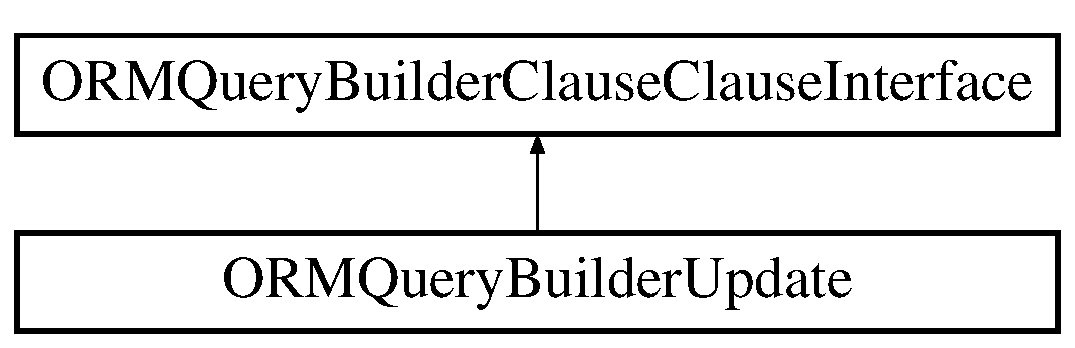
\includegraphics[height=2.000000cm]{classORM_1_1QueryBuilder_1_1Update}
\end{center}
\end{figure}
\subsection*{Public Member Functions}
\begin{DoxyCompactItemize}
\item 
{\bfseries from} (\$table)\hypertarget{classORM_1_1QueryBuilder_1_1Update_a627f95aa098ccd1fef6020e400304b0c}{}\label{classORM_1_1QueryBuilder_1_1Update_a627f95aa098ccd1fef6020e400304b0c}

\item 
{\bfseries set} (\$values)\hypertarget{classORM_1_1QueryBuilder_1_1Update_a55a6e2addd302018fb1fbf2581b2d209}{}\label{classORM_1_1QueryBuilder_1_1Update_a55a6e2addd302018fb1fbf2581b2d209}

\item 
{\bfseries to\+Sql} ()\hypertarget{classORM_1_1QueryBuilder_1_1Update_a65eb228cb7cc55c85920fee639e40c57}{}\label{classORM_1_1QueryBuilder_1_1Update_a65eb228cb7cc55c85920fee639e40c57}

\end{DoxyCompactItemize}


The documentation for this class was generated from the following file\+:\begin{DoxyCompactItemize}
\item 
app/orm/src/\+Query\+Builder/Update.\+php\end{DoxyCompactItemize}

\hypertarget{classORM_1_1Persistence_1_1UpdatePersist}{}\section{O\+RM\textbackslash{}Persistence\textbackslash{}Update\+Persist Class Reference}
\label{classORM_1_1Persistence_1_1UpdatePersist}\index{O\+R\+M\textbackslash{}\+Persistence\textbackslash{}\+Update\+Persist@{O\+R\+M\textbackslash{}\+Persistence\textbackslash{}\+Update\+Persist}}
Inheritance diagram for O\+RM\textbackslash{}Persistence\textbackslash{}Update\+Persist\+:\begin{figure}[H]
\begin{center}
\leavevmode
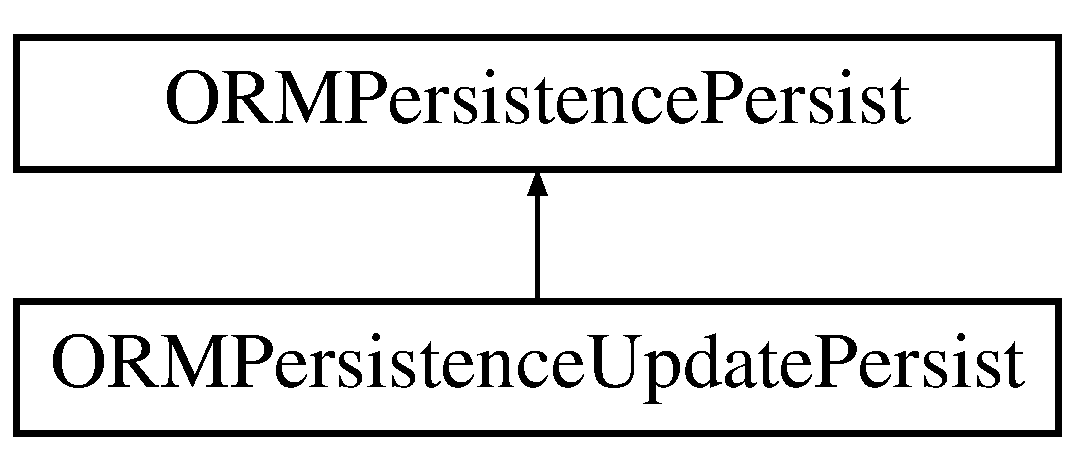
\includegraphics[height=2.000000cm]{classORM_1_1Persistence_1_1UpdatePersist}
\end{center}
\end{figure}
\subsection*{Public Member Functions}
\begin{DoxyCompactItemize}
\item 
{\bfseries analyze} ()\hypertarget{classORM_1_1Persistence_1_1UpdatePersist_a4eaa1b3bc00c1ab9bf705285ee30b394}{}\label{classORM_1_1Persistence_1_1UpdatePersist_a4eaa1b3bc00c1ab9bf705285ee30b394}

\end{DoxyCompactItemize}
\subsection*{Additional Inherited Members}


The documentation for this class was generated from the following file\+:\begin{DoxyCompactItemize}
\item 
app/orm/src/\+Persistence/Update\+Persist.\+php\end{DoxyCompactItemize}

%--- End generated contents ---

% Index
\backmatter
\newpage
\phantomsection
\clearemptydoublepage
\addcontentsline{toc}{chapter}{Index}
\printindex

\end{document}
